\chapter{Personendetektion}
\label{chap:Personendetektion}

Auf der Grundlage der vorherigen Kapitel wird nun mittels einem neuronalen Netzwerks eine Personenerkennung erstellt. Dieser Abschnitt beschreibt das Vorgehen, um die Anzahl Personen in einem Aufzug zu erkennen. In einem ersten Schritt wird die Verarbeitung der Rohdaten aufgezeigt. Anschliessend werden diverse Ansätze erläutert, um die Datensätze zu verbessern. Für den Auswertealgorithmus wurden drei unterschiedliche Aufzüge evaluiert und für jeden Aufzug ein eigenes Profil erstellt. 

\section{Datenverarbeitung}
\label{Datenverarbeitung}

Mittels dem erstellten C-Programm ConvertValue\_V2 lassen sich die Rohdaten in \ac{CSV}-Files konvertieren. Dabei wird über die USB-Schnittstelle mit dem Open-Source Terminal-Programm H-Term die \ac{ASCII}-Rohdaten ausgelesen [\protect\cite{HTERM}].
Das Programm H-Term fügt zudem jedem Datensatz den aktuellen Zeitstempel an. In Abbildung \ref{fig:Dataframe} ist der Aufbau des Datenframes ersichtlich.

\begin{figure}[H]
	\centering
	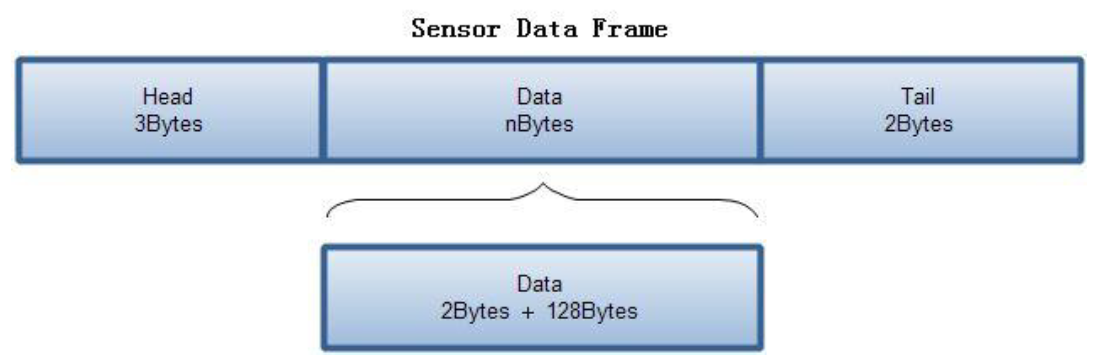
\includegraphics[width=0.5\textwidth]
	{fig/Dataframe}
	\caption[Datenframe des Eval Boards]{Datenframe des Eval Boards}
	\label{fig:Dataframe}
\end{figure}

Zum Vergleich ist nachfolgend ein einzelnes Datenframe dargestellt. Der Header besteht aus der Zeichenfolge *** und wird zur Synchronisation benötigt. Danach folgen 2 Byte für den Thermistorwert (\textcolor{blue}{blau}) und 128 Byte für die 64 Pixelwerte. Als Schluss wird die Zeile mit \textbackslash n \textbackslash r beendet.

17:34:04.009: \\
***\textcolor{blue}{‘ r} h m l h f d \^ \space \space Z ` k f i g b Z Z X Z [ \_ a W X Y X Y V U T T U W U R R T U S U T XT R Q R R T V R R P S P U U V U Q P P O P Q V  \textbackslash n \textbackslash r \\

Mit dem ConvertValue\_V2 werden diese \ac{ASCII}-Zeichen in die entsprechenden Fliesskommazahlen umgewandelt und formatiert. Nachfolgend ist die entsprechende Ausgabe ersichtlich.

26.000 ,27.250 ,27.000 ,26.000 ,25.500 ,25.000 ,23.500 ,22.500 ,24.000 ,26.750 ,25.500 ,26.250 ,25.750 ,24.500 ,22.500 ,22.500 ,22.000 ,22.500 ,22.750 ,23.750 ,24.250 ,21.750 ,22.000 ,22.250 ,22.000 ,22.250 ,21.500 ,21.250 ,21.000 ,21.000 ,21.250 ,21.750 ,21.250 ,20.500 ,20.500 ,21.000 ,21.250 ,20.750 ,21.250 ,21.000 ,22.000 ,21.000 ,20.500 ,20.250 ,20.500 ,20.500 ,21.000 ,21.500 ,20.500 ,20.500 ,20.000 ,20.750 ,20.000 ,21.250 ,21.250 ,21.500 ,21.250 ,20.250 ,20.000 ,20.000 ,19.750 ,20.000 ,20.250 ,21.500 ,\textcolor{blue}{25.0625} ,17:34:04.009

Durch das Programm H-Term sind bei der Messung sporadisch fehlerhafte Datenströme entstanden, da der mitgesendete Zeitstempel erst nach dem Header eingefügt wurde. Dies verursachte bei der Konvertierung negative Temperaturwerte, welche von Hand korrigiert werden mussten. 


\section{Datenmanipulation mittels Interpolation}
\label{sec:Datenmanipulation}

Die Auflösung von 8x8 Pixel bietet nur begrenzte Wärmebildinformationen über die Anzahl Personen in einem Aufzug. Daher wurde in MATLAB mehrere Interpolationsverfahren benutzt, um die Auflösung, und somit die Wärmebildinformationen, zu vergrössern. Im Zusammenhang mit den Pixelwerten eignet sich das bikubische oder das lanczossche Interpolationsverfahren [\protect\cite{Interpol}]. Beim bikubischen Ansatz werden die berechneten Pixel gleichmässig interpoliert. Beim lanczosschen Interpolationsverfahren werden wärmere Gebiete stärker vom kühleren Hintergrund getrennt. Bei einer Interpolation von 8x8 Pixel auf 32x32 Pixel nähern sich die Werte beider Verfahren sehr stark an, da die originalen Wärmebildinformationen begrenzt sind. In Abbildung \ref{fig:interpol1} und \ref{fig:interpol2} sind das Orginalframe, indem sich drei Personen befinden, und die lanczossche Interpolation dargestellt.


\begin{figure}[!ht]
	\centering
	\begin{minipage}[c]{0.49\linewidth}
	\centering
	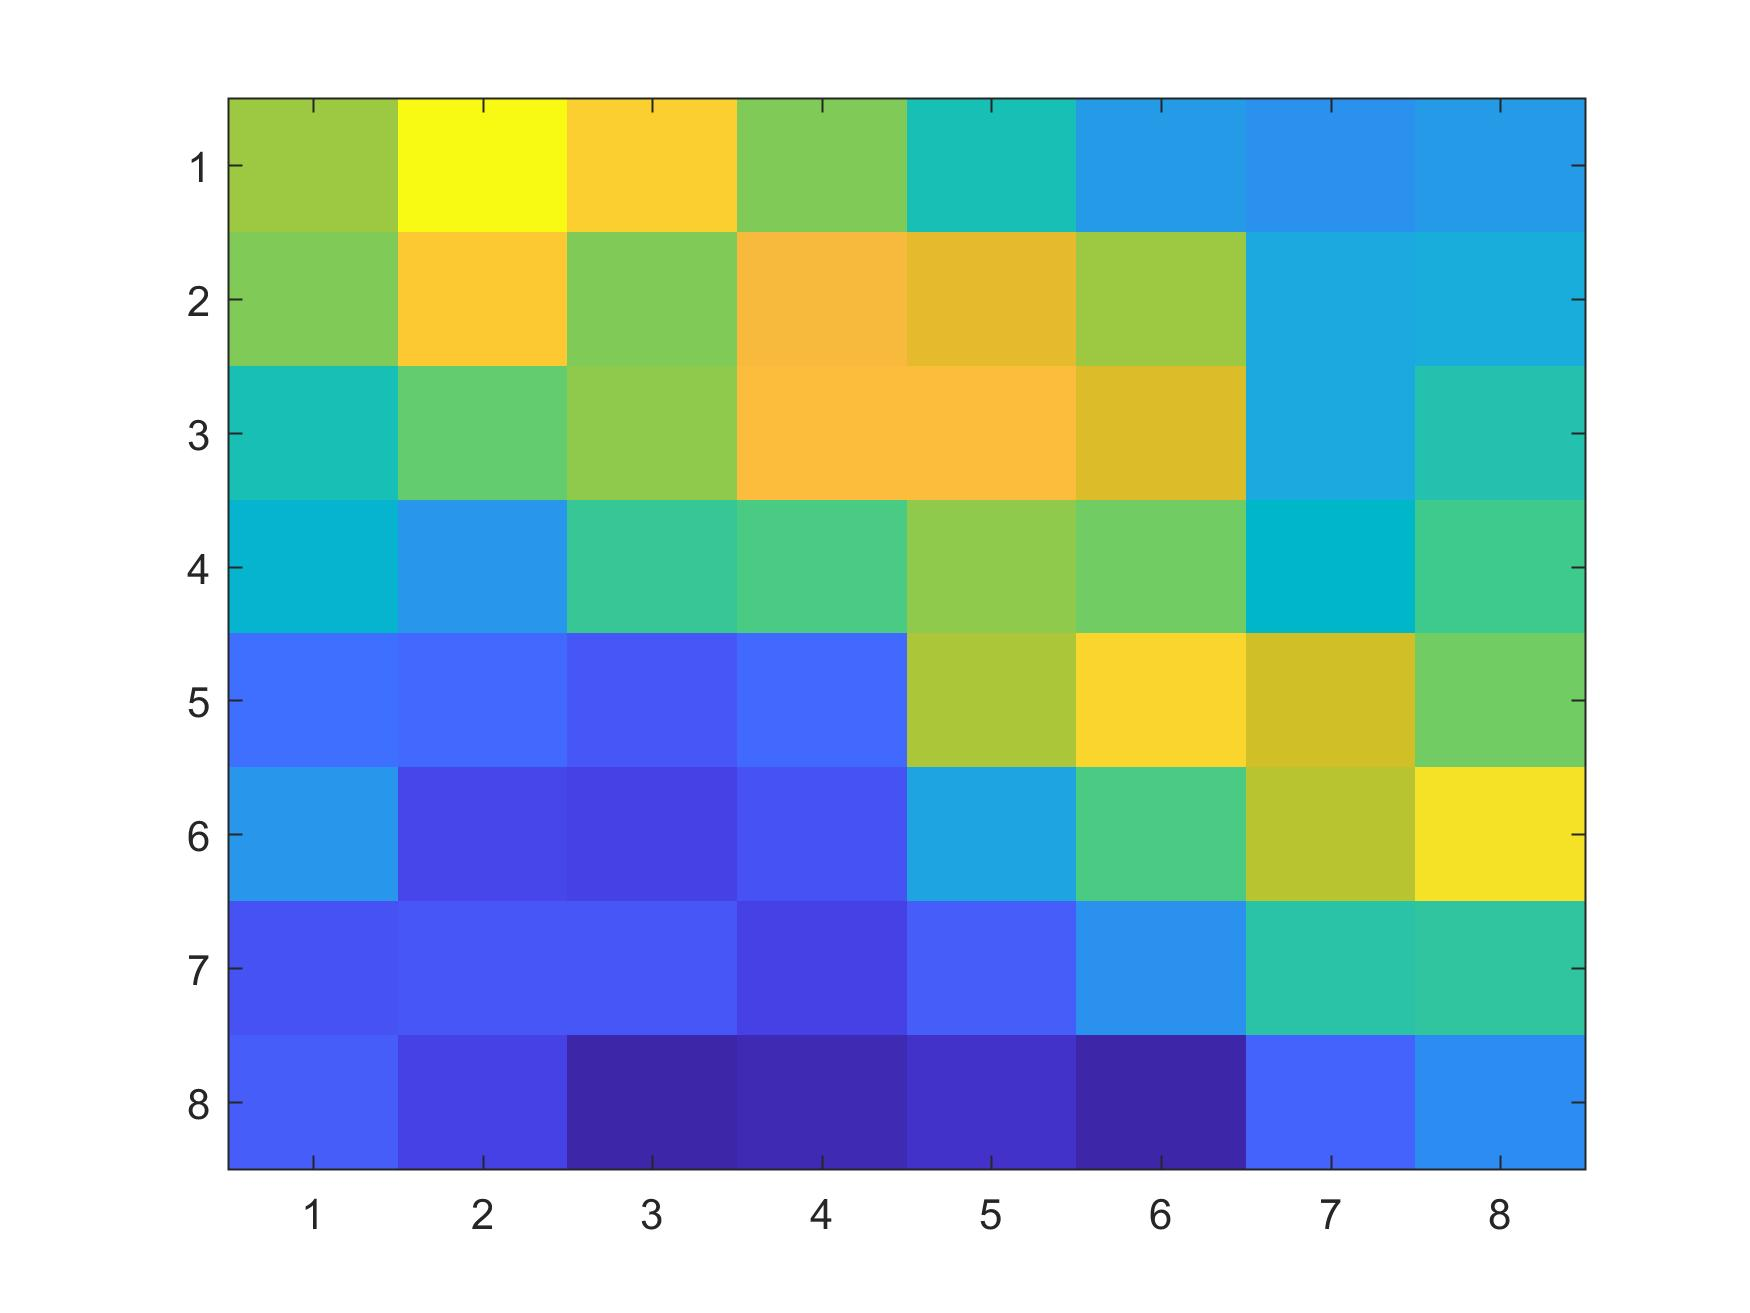
\includegraphics[width=1.0\linewidth]{fig/interpol_1}
	\caption[Originalframe]{Originalframe}
	\label{fig:interpol1}
	\end{minipage}
	\begin{minipage}[c]{0.49\linewidth}
		\centering
	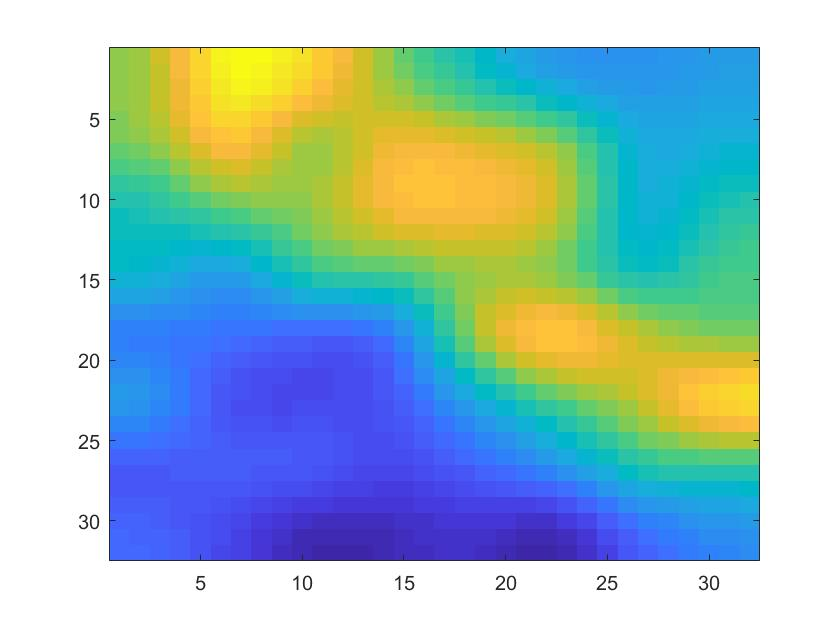
\includegraphics[width=1.0\linewidth]{fig/interpol_2}
	\caption[Lanczossche Interpolation]{Lanczossche Interpolation}
	\label{fig:interpol2}
	\end{minipage}
\end{figure}

In Hinsicht auf das neuronale Netzwerk bieten vor allem grössere Auflösungen mehr Spielraum für das \ac{CNN}. Es können so grössere Filter verwendet werden, damit mehr Eigenschaften\footnote[23]{Sogenannte Features} identifiziert werden. Die Auflösung gibt zudem auch die Tiefe des neuronalen Netzwerks vor. Je weniger Bildinformationen zur Verfügung stehen, desto weniger gewinnbringend sind zusätzliche Ebenen im neuronalen Netzwerk. 

Weiter kann man davon ausgehen, dass die Hintergrundtemperatur und die Thermistorwerte, sofern keine Störquellen einwirken, identisch sind. Damit lässt sich eine Bildkorrektur durchführen. Wird angenommen, dass Personen wärmer sind als die Umgebung, dann lässt sich das Bild auf die entsprechenden Pixel filtern. Es entsteht ein binäres Wärmebild, welches die Personen hervorhebt. 

\begin{figure}[H]
	\centering
	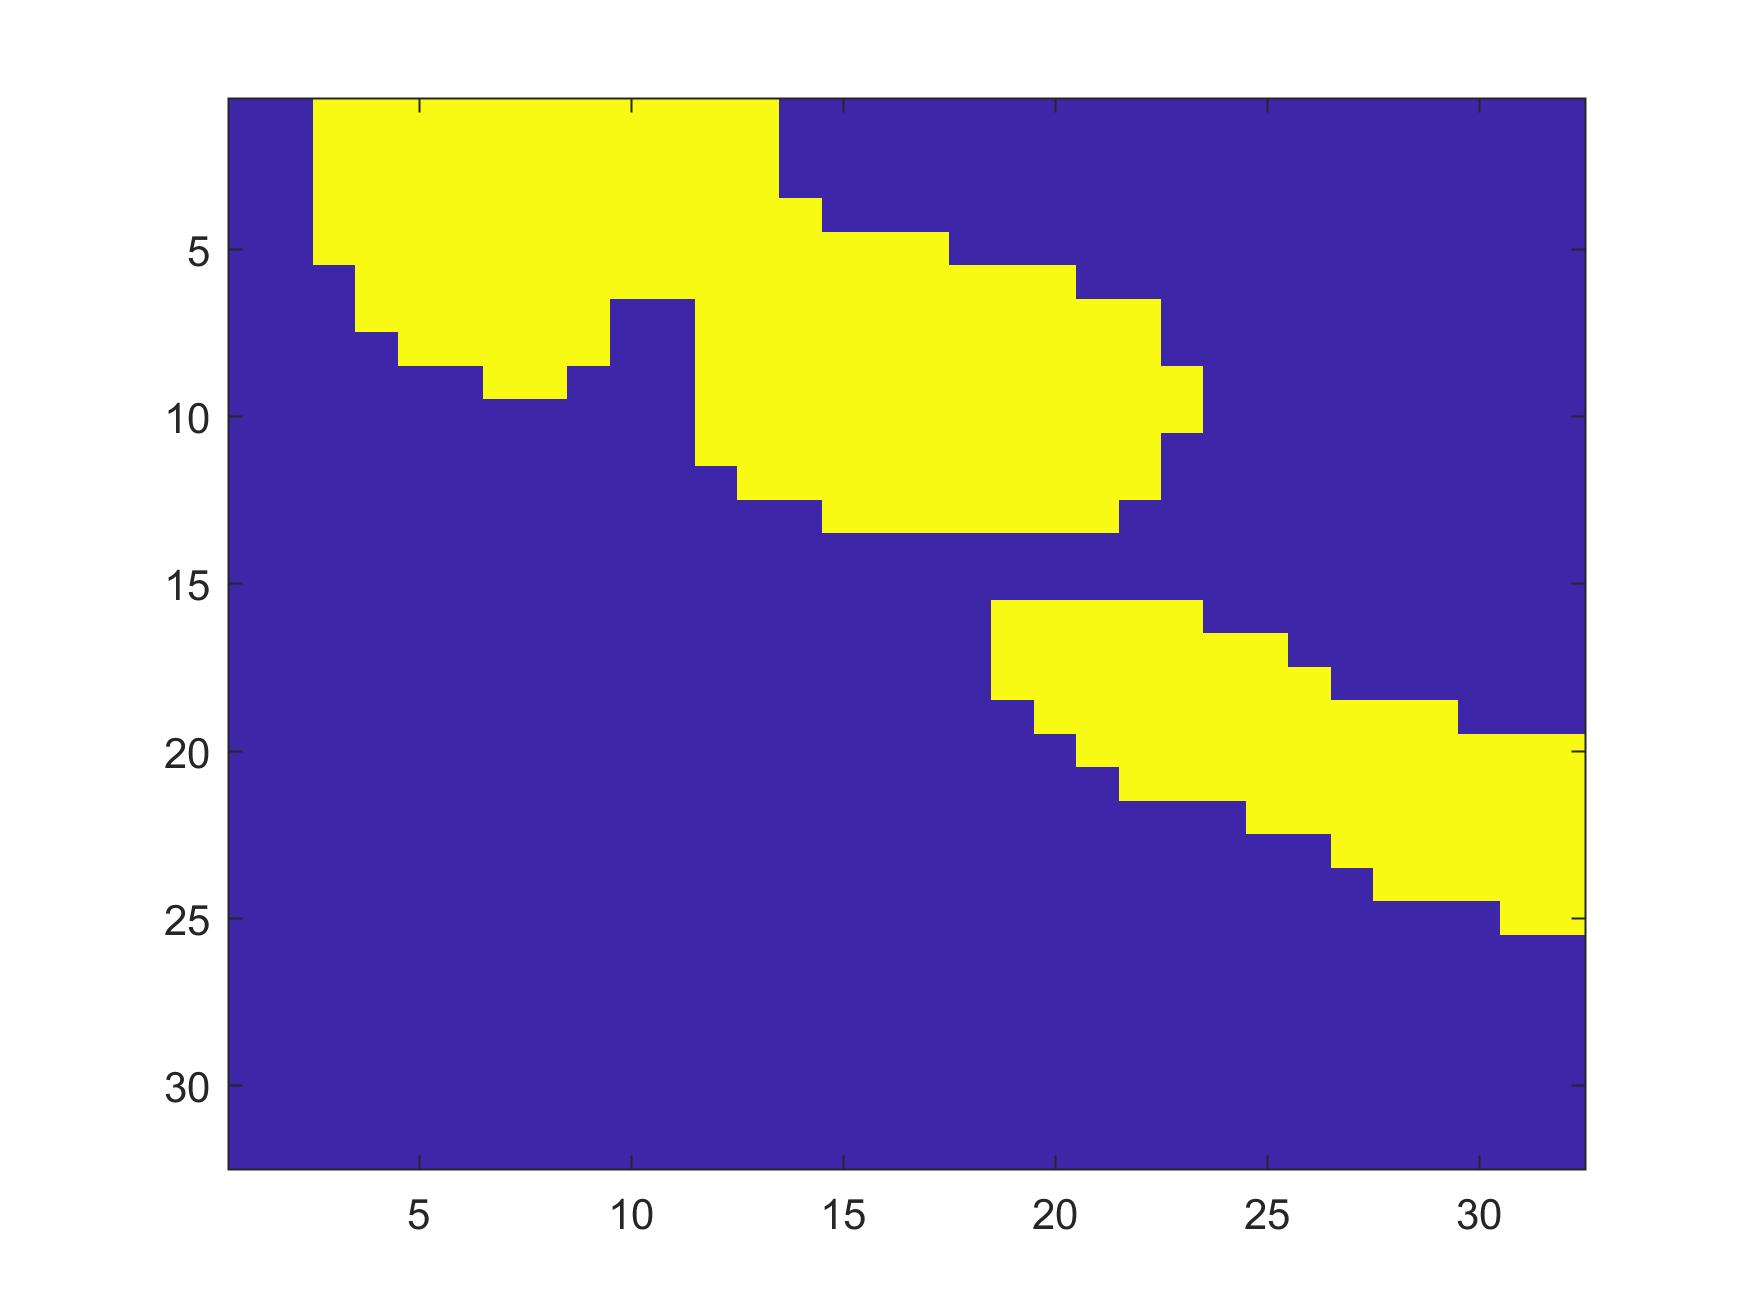
\includegraphics[width=0.5\linewidth]{fig/interpol_3}
    \caption[Temperaturkorrektur]{Temperaturkorrektur}
   \label{fig:interpol3}
\end{figure}

Mit diesem binären Filter können die Wärmemuster, die Personen besitzen, vereinfacht betrachtet werden. Dieser Ansatz bedingt jedoch, dass die Personen zu jeder Zeit höhere Temperaturen besitzen als die Umgebungstemperatur. Dies kann nicht jederzeit garantiert werden, daher wurde dieser Ansatz nicht weitergeführt.

Nachteilig ist bei beiden Ansätzen, dass die Wärmebildinformationen mit zunehmender Grösse zum Teil stark verfälscht werden oder verloren gehen, da sich die interpolierten Pixel nur rechnerisch abschätzen lassen. Es wurde daher entschieden, die Auflösung bei den unverfälschten, originalen Frames zu belassen. Es werden keine Bildinformationen manipuliert oder gehen verloren, jedoch ist die Tiefe des neuronalen Netzwerks beschränkt.

\section{Symmetrische Erweiterung}
\label{sec:Symmetrische Erweiterung}

Um die Messdaten zu vergrößern wurden diese mit deren Symmetrien erweitert. Dafür wurde für das jeweilige Profil je ein Python-Programm rotate\_and\_swap\_ProfilX.py\footnote[24]{Im digitalen Anhang \ref{AnhangDig} angefügt}  geschrieben, welches alle Frames der Datensätze symmetrisch erweitert. Es lassen sich zusätzlichen Frames bilden, welche in den nachfolgenden Abbildungen \ref{fig:original} und \ref{fig:rotated} dargestellt sind.

\begin{figure}[!ht]
	\centering
	\begin{minipage}[c]{0.35\linewidth}
	\centering
	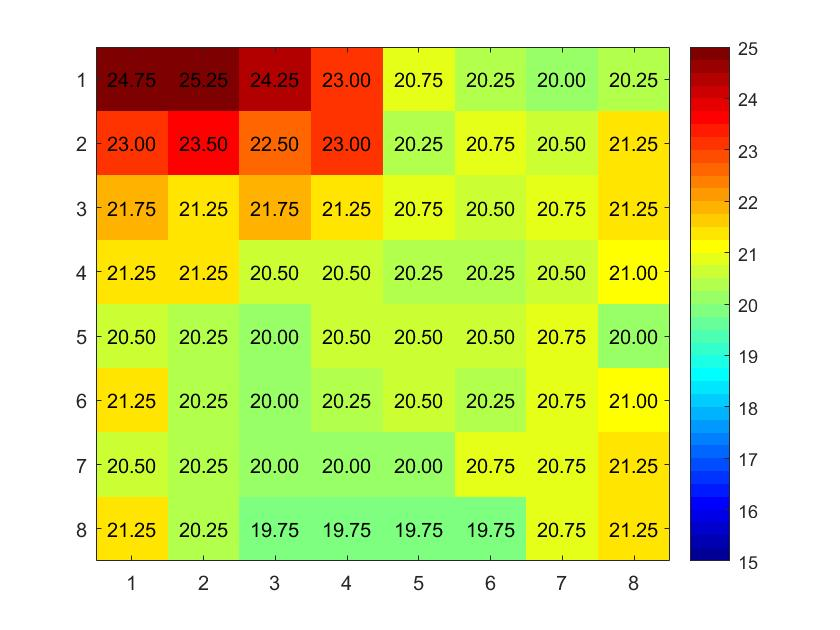
\includegraphics[width=.8\linewidth]{fig/original}
	\caption[Originales Frame]{Originales Frame}
	\label{fig:original}
	\end{minipage}
	\hfill
	\begin{minipage}[c]{0.6\linewidth  }
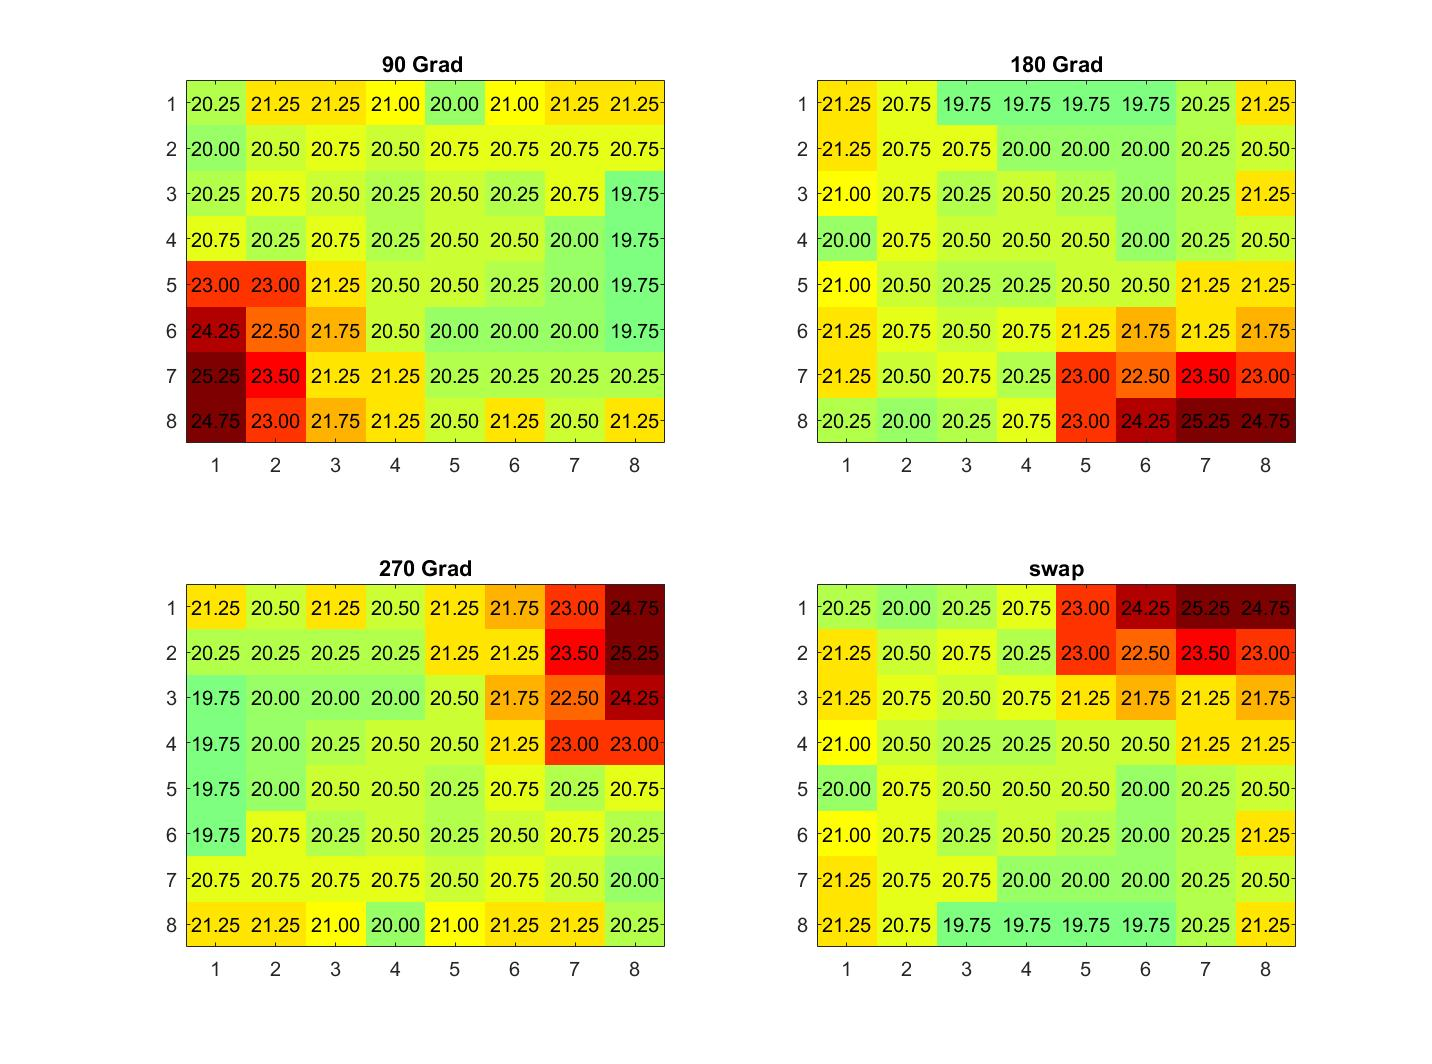
\includegraphics[width=1\linewidth]{fig/rotated}
\caption[Rotierte und gespiegelte Frames]{Rotierte und gespiegelte Frames}
\label{fig:rotated}
	\end{minipage}
\end{figure}


Durch die Erweiterung konnten die Messdaten um den Faktor 5 vergrößert und nicht vermessenen Positionen nachträglich generiert werden. Mit den Messstandorten A bis L und den generierten Erweiterungen stehen eine Vielzahl an Varianten zur Verfügung. 


\section{Profilbildung}
\label{sec:Profilbildung}

Mit den Python-Skripts rawDataMergeV3\_ProfilX.py\footnote[25]{Im digitalen Anhang \ref{AnhangDig} angefügt} werden die einzelnen Messungen zu einem Datenset zusammengestellt. Jedem Frame wird eine weitere Spalte, die die richtige Anzahl Personen im Frame angibt, mitgegeben. Die zusammengefügten Datensätze wurden nach den drei vermessenen Aufzugsprofilen erstellt. Ein Überblick über die Messumgebungsparameter des jeweiligen Profils ist in Anhang \ref{AnhangD} angefügt.

Es lassen sich  individuell weitere Files hinzufügen oder entfernen. Die  Tabelle \ref{tab:Profilbildung} zeigt, aus welchen Frames die Profile zusammengesetzt sind.

\begin{table}[H]
	\centering
	\caption[Zusammensetzung  der Profile in {[Frames]}]{Zusammensetzung  der Profile in {[Frames]}}
	\label{tab:Profilbildung}
	\begin{tabular}{|c|c|c|c|c|c|c|}
		\hline
		\rowcolor[HTML]{9B9B9B} 
		\multicolumn{1}{|l|}{\cellcolor[HTML]{9B9B9B}}                   & \multicolumn{1}{l|}{\cellcolor[HTML]{9B9B9B}\textbf{0 Personen}} & \textbf{1 Person} & \textbf{2 Personen} & \textbf{3 Personen} & \textbf{4 Personen} & \textbf{Gesamt} \\ \hline
		\cellcolor[HTML]{9B9B9B}\textbf{Profil 1}                         & 21632                                                            & 42129             & 46826               & 23943               & 17406               & 151936          \\ \hline
		\cellcolor[HTML]{9B9B9B}\textbf{Profil 2}                        & 21632                                                            & 42284             & 47736               & 23108               & 18421               & 153181          \\ \hline
		\cellcolor[HTML]{9B9B9B}{\color[HTML]{333333} \textbf{Profil 3}} & 21632                                                            & 43479             & 47631               & 23933               & 17786               & 154461          \\ \hline
	\end{tabular}
\end{table}

Neben den drei Profilen wurde ein Testprofil erstellt, welches keine Frames der anderen drei Profile verwendet. Dieses Testprofil besitzt hauptsächlich Ausnahmesituationen, die für den Algorithmus schwieriger zu erkennen sind. Dabei wurden folgende Ausnahmesituationen angewendet:

\begin{itemize}
	\item Nahe nebeneinander stehende Personen 
	\item Personen am Rand des Messbereichs
	\item Störquellen im Messbereich
	\item Objekte mit Temperaturdifferenzen
\end{itemize}

Es wurden dafür auch Messdaten aus Kapitel \ref{chap:Testphasen} verwendet. Die Tabelle \ref{tab:Testprofil} zeigt die Zusammensetzung des Testprofils auf.

\begin{table}[H]
	\centering
	\caption[Zusammensetzung  des Testprofils in {[Frames]}]{Zusammensetzung  des Testprofils in [Frames]}
	\label{tab:Testprofil}
	\begin{tabular}{|c|c|c|c|c|c|c|}
		\hline
		\rowcolor[HTML]{9B9B9B} 
		\multicolumn{1}{|l|}{\cellcolor[HTML]{9B9B9B}}                   & \multicolumn{1}{l|}{\cellcolor[HTML]{9B9B9B}\textbf{0 Personen}} & \textbf{1 Person} & \textbf{2 Personen} & \textbf{3 Personen} & \textbf{4 Personen} & \textbf{Gesamt} \\ \hline
		\cellcolor[HTML]{9B9B9B}\textbf{Testprofil}                         & 14316                                                          & 3423             & 621               & 3803                & 2495               & 24658          \\ \hline
	\end{tabular}
\end{table}

\section{Aufbau des Convolution Neural Network}
\label{AufbauConv}

Für das neuronale Netzwerk wurde ein zweistufiges Python-Skript geschrieben, welches vom Beispiel des \ac{MNIST Dataset} und des Hvass-Labs adaptiert wurde [\protect\cite{Tensorflow}][\protect\cite{HVASS}].

Im Teil Input\_data.py wurde eine Klasse Dataset erstellt, welche alle nötigen Funktionen besitzt, um die Frames aus dem \ac{CSV}-File soweit vorzubereiten, damit diese dem neuronalen Netzwerk als Input übergeben werden kann. 

In dieser Klasse lassen sich die jeweiligen Test- und Trainingsets wählen. Daneben kann ein zusätzliches Validierungsset aus dem Trainingsset extrahiert werden. Dieses wird benötigt, um das zu trainierende Modell bestmöglich anzupassen\footnote[26]{Auch bekannt als model fitting}. Nähere Erläuterungen zu Training und Validierung folgen im Unterkapitel \ref{TrainingValidierung}.

Das \ac{CNN} wurde im Teil Personendetektion\_Modelling\_V3\_ProfilX.py\footnote[27]{im digitalen Anhang \ref{AnhangDig} angefügt} implementiert. Daneben besitzt dieses Python-Skript einige Hilfsfunktionen, welche für das Training und die Validierung nötig sind.

Anfänglich wurde mit der Tiefe des Netzwerks variiert, dabei wurde die Tiefe stetig vergrössert bis keine Verbesserungen mehr erkennbar waren. Es stellte sich heraus, dass ein dreistufiges Netzwerk die besten Ergebnisse liefert.

Das Netzwerk besteht aus mehreren Teilblöcken, die üblicherweise sequentiell hintereinander geschaltet sind. Dabei wird jedes Frame einzeln dem \ac{CNN} übergeben und ausgewertet. Nachfolgend sind die Funktionen der Teilblöcke kurz beschrieben, wobei nähere Erläuterungen online\footnote[28]{Unter www.tensorflow.org } zu finden sind.

\textbf{Convoluton Layer:} Filtermatrizen die entsprechend der Einstellung durch das gesamte vorhandene Bild iterieren, um Features zu identifizieren.   \\
\textbf{Polling Layer:} Überflüssige Informationen werden entfernt und das Frame wird verkleinert.   \\
\textbf{Fully-connected Layer:} Werden zur Klassifizierung am Ende des Netzwerks angewendet, indem mehrere Verknüpfungen aktiviert werden. Aus den aktivierten Verknüpfungen wird der entsprechende Output ausgegeben.  

Das erstellte Netzwerk ist funktionell in Abbildung \ref{fig:CNN} dargestellt.
\begin{figure}[H]
	\centering
	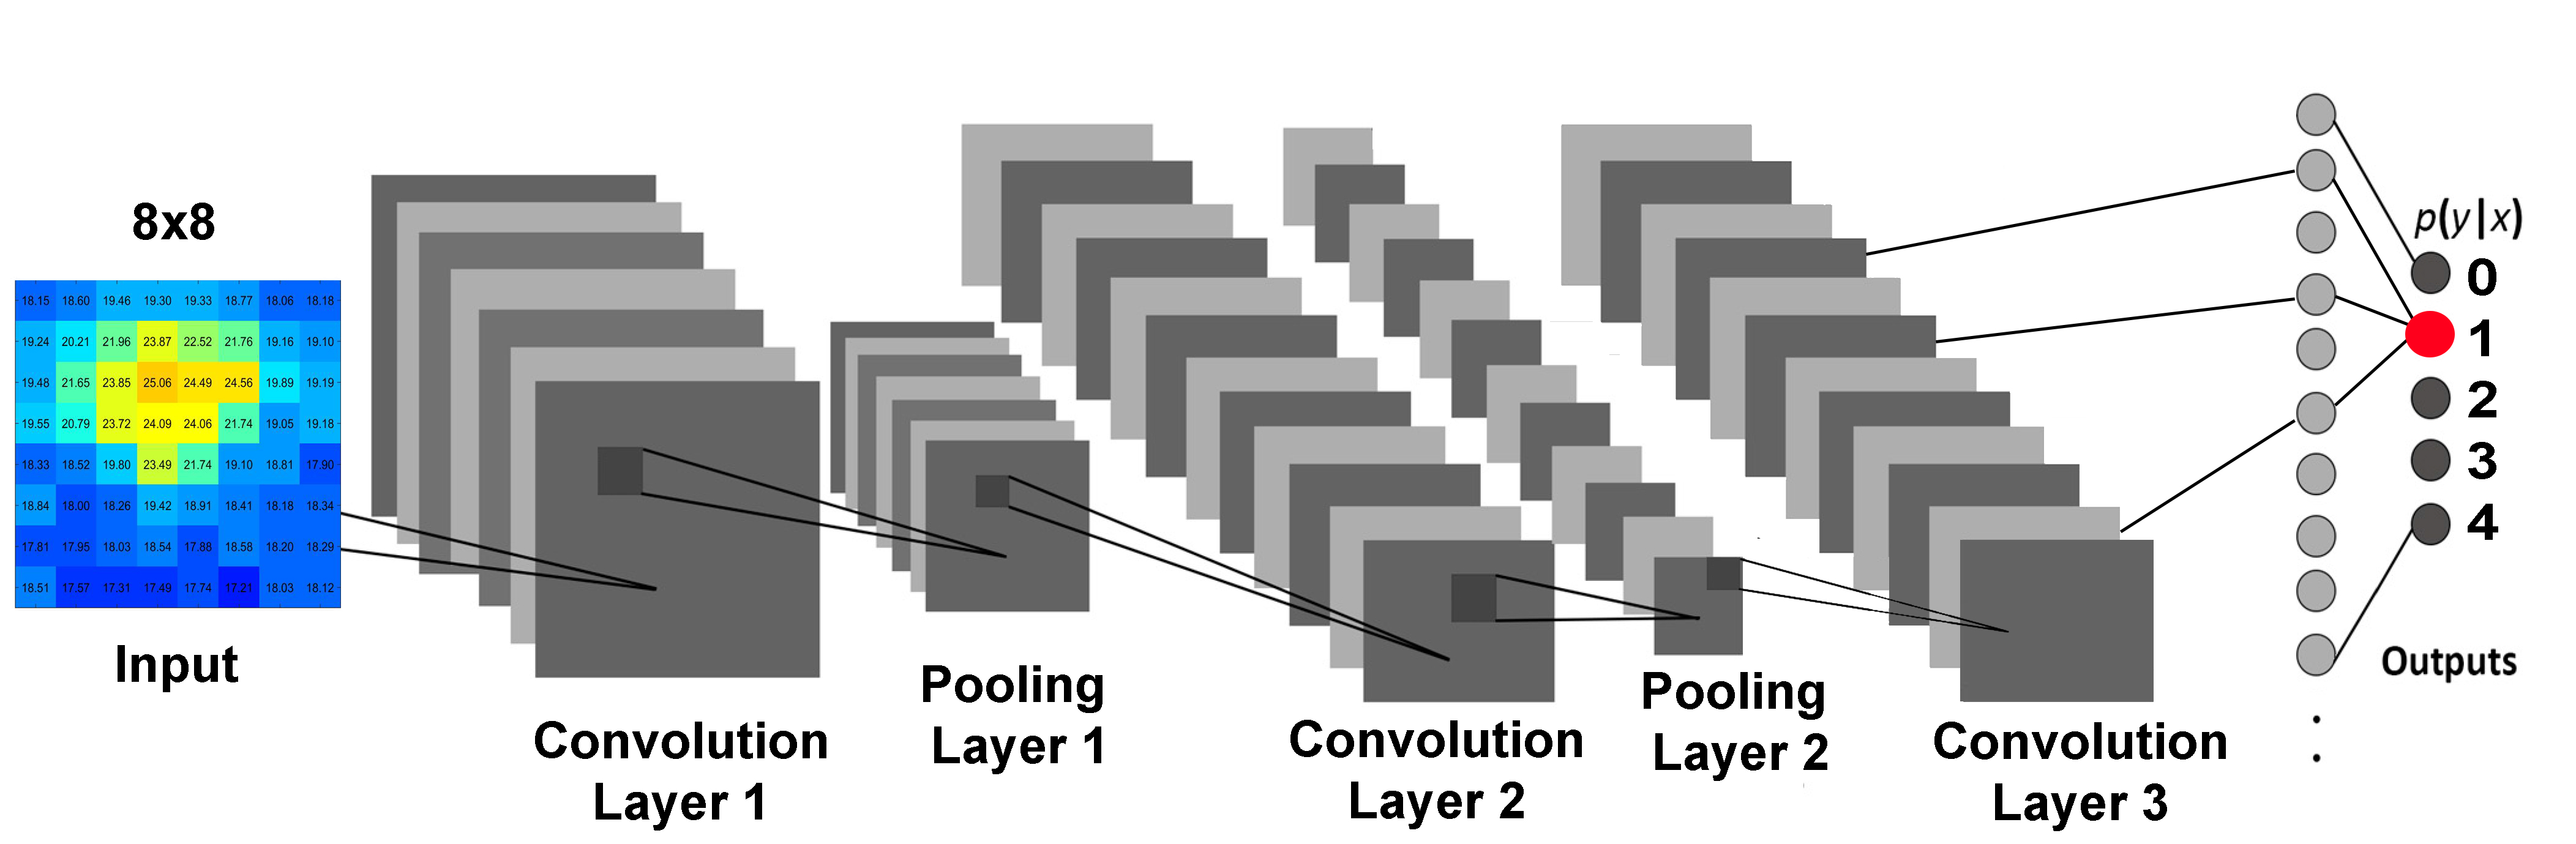
\includegraphics[width=1\textwidth]
	{fig/CNN_broschuere.jpg}
	\caption[Aufbau des Convolutional Neural Network]{Aufbau des Convolutnional Neural Network}
	\label{fig:CNN}
\end{figure}

Tensorflow bietet verschiedene Abstraktionsstufen dieser Blöcke. Dabei wurde mit der tf.Layer Klasse gearbeitet.
Für die Convolution Layer wurden eine 6x6 und zwei 3x3 Matrizen verwendet. Weitere eingestellte Parameter sind im  Anhang \ref{AnhangDig} einsehbar.

\newpage
\section{Training und Validierung}
\label{TrainingValidierung}

Im Python-Skript Personendetektion\_Modelling\_V3\_ProfilX.py wurde das \ac{CNN} mit den erstellen Profilen trainiert. Es wurde nach dem üblichen Trainingsverfahren für neuronale Netzwerke trainiert.

Dafür werden ständig neue zufällige Frames aus dem Datenset zu einem Batch\footnote[29]{Zu Deutsch: Stapel} zusammengefügt und iterativ dem \ac{CNN} übergeben. Während den Iterationen werden mit den Labels ständig Soll-Ist-Vergleiche durchgeführt und die Parameter der Layer automatisch verbessert. 
Für den Optimierungsalgorithmus wurden mehrere verschiedene Algorithmen ausprobiert. Die besten Ergebnisse konnten mit dem AdamOptimizer erzielt werden. Dafür wurden die standardmäßigen Parameter von Tensorflow übernommen.

In Abbildung \ref{fig:traininsverlauf} ist die prozentuale Übereinstimmung der Frames mit einer Batchgrösse von 1000 Frames in Abhängigkeit der Anzahl Iterationen abgebildet. Dabei wird das Trainingsset und das Vaildierungsset verwendet. Sie zeigen die aktuellen Übereinstimmungen an. 

\begin{figure}[H]
	\centering
	\caption[Trainingsverlauf Profil 1]{Trainingsverlauf Profil 1}
	\label{fig:traininsverlauf}
	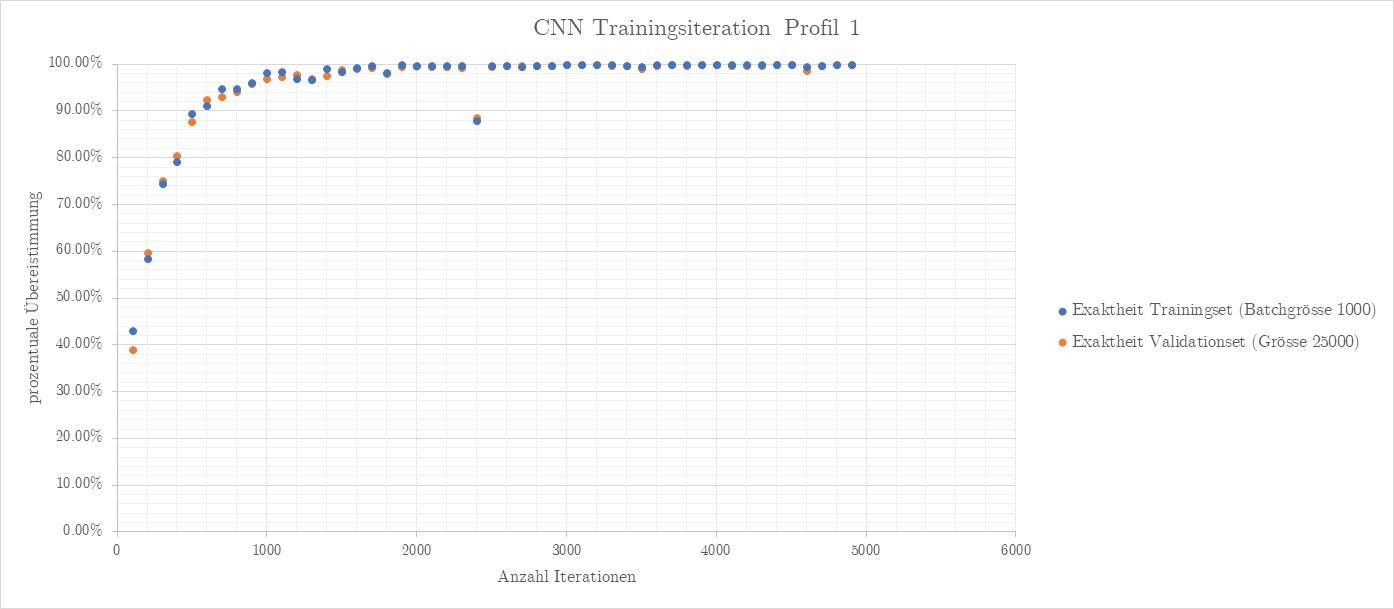
\includegraphics[width=1.0\linewidth]{fig/Traininsverlauf}
\end{figure}

Die Übereinstimmung steigt anfänglich stark an und konvergieren nahe zu 100\%. Das Validationsset besitzt eine sehr ähnliche Übereinstimmung. Dies liegt daran, dass es sich um 25000 zufällige Frames handelt, die aus dem Trainingsset entnommen wurden. Während den Iterationen werden mit der Saver-Klasse von Tensorflow die besten prozentualen Ergebnisse\footnote[30]{Übereistimmung: Training: 100.00\%, Validierung 99.92\%}  in ein Modell gespeichert. Diese können dann weiter verwendet werden. Je nach Grösse der Parameter kann diese Berechnung bis zu mehreren Stunden\footnote[31]{Abhängig von der Rechenleistung des Computers} dauern. 


\section{Ergebnisse}
\label{sec:Ergebnisse}

In diesem Unterkapitel werden die Resultate der Profile ausgewertet und durch eine Confusion Matrix dargestellt. Diese gibt Auskunft, welche Vorhersagen durch das erstellte Modell richtig oder fehlerhaft detektiert wurden. Die Confusion Matrix gibt dabei prozentual und effektiv die Anzahl der klassifizierten Frames wieder. 


\subsection{Profil 1}
\label{subsec:Profil1}
Im Vergleich mit den anderen zwei Profilen konnten mit dem Profil 1 die besten Ergebnisse erzielt werden. Daher wurde das endgültige Model mit dem Datenset des Profils 1 trainiert. Die Abbildung \ref{fig:profil1} zeigt die Übereinstimmung des trainierten Modells, wenn das Model auf das eigene Datenset getestet wird. 


\begin{figure}[H]
	\centering
	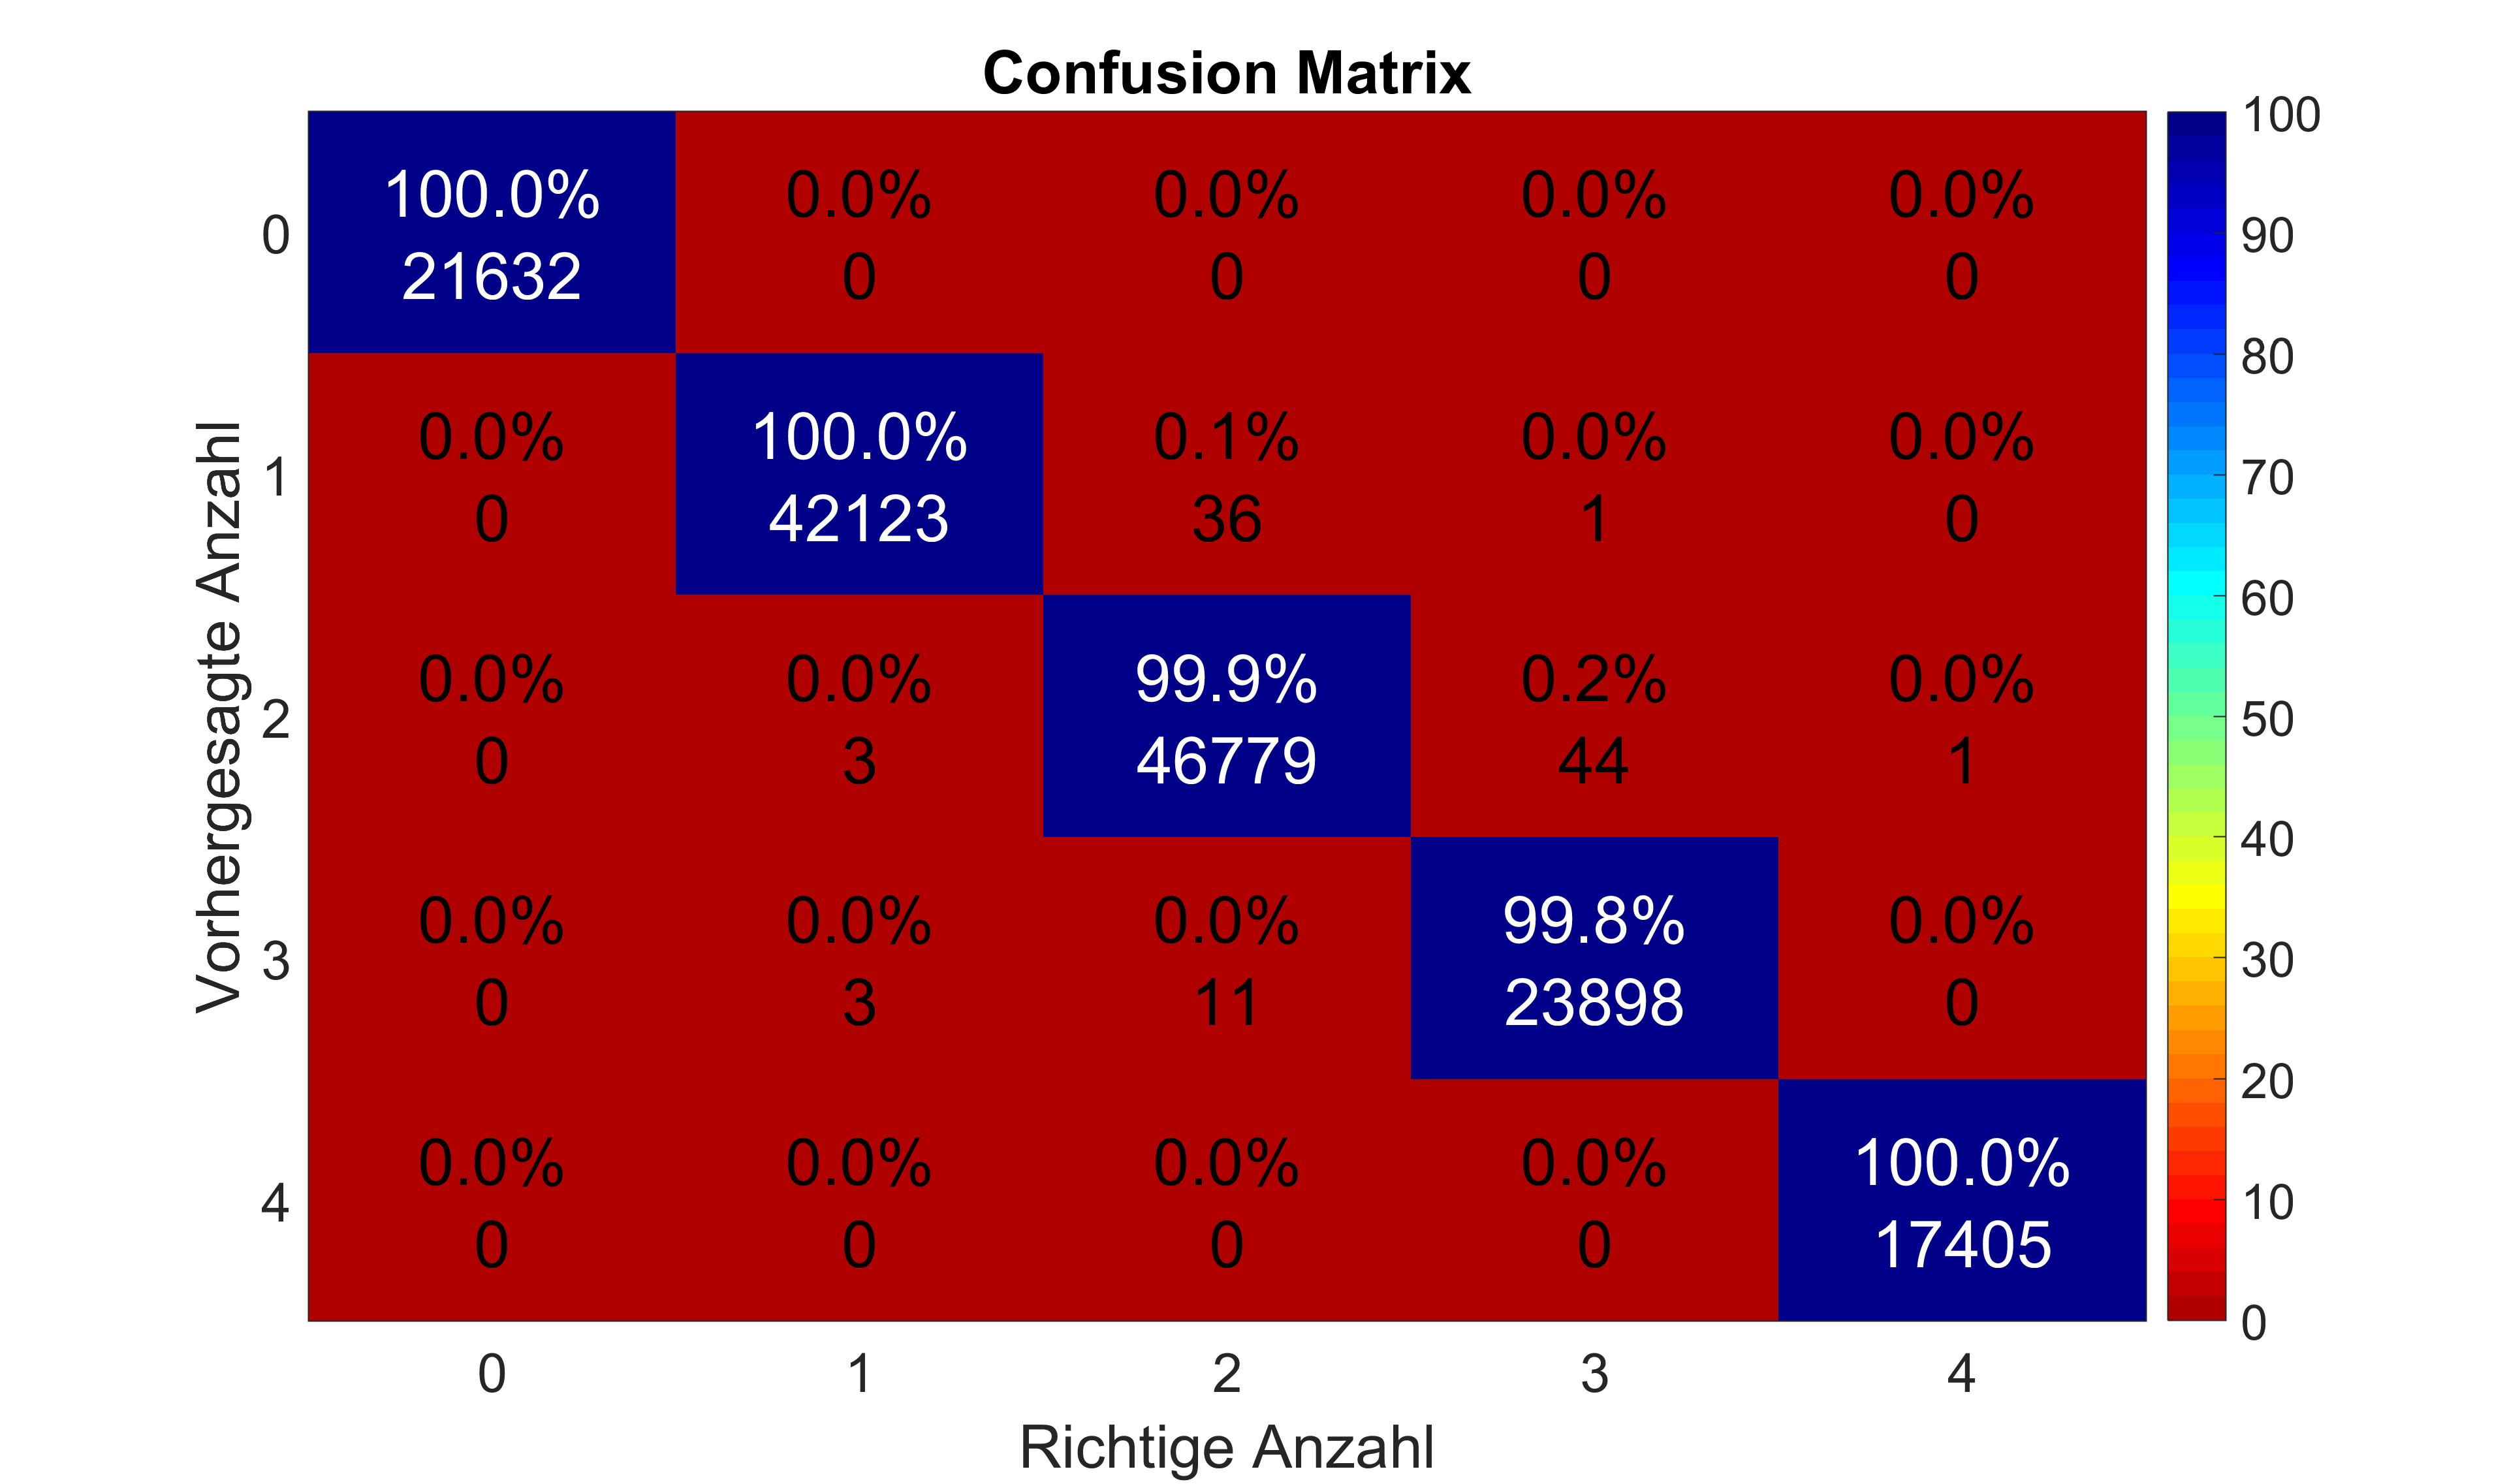
\includegraphics[width=0.55\linewidth]{fig/Profil_1m}
	\caption[Confusion Matrix Profil 1]{Confusion Matrix Profil 1}
		\label{fig:profil1}

\end{figure}

 Es ist naheliegend, dass praktisch alle vorhergesagten Frames richtig klassifiziert wurden, weil das Modell auf diese Frames trainiert wurde. Die grössten Verfehlungen liegen bei der Klassifizierung von zwei und drei Personen. Es wurden 44 Frames als Zwei klassifiziert, wobei sich richtigerweise drei Personen im Messbereich befanden. Im Verhältnis zu den insgesamt 151935 Frames sind dies jedoch sehr tiefe Werte.

\subsection{Profil 2}
\label{subsec:Profil2}
Mit dem Profil 2 wurden im Allgemeinen die schlechtesten Ergebnisse erzielt. Bei der Betrachtung der fehlerhaften Frames, wurde festgestellt, dass es einige Frames gibt in denen bei den drei Personen Frames eine Person kaum im Messbereich stand und dadurch schwieriger zu identifizieren ist. Dies ist auch in der folgenden Confusion Matrix in Abbildung \ref{fig:profil2} ersichtlich.

\begin{figure}[H]
	\centering
	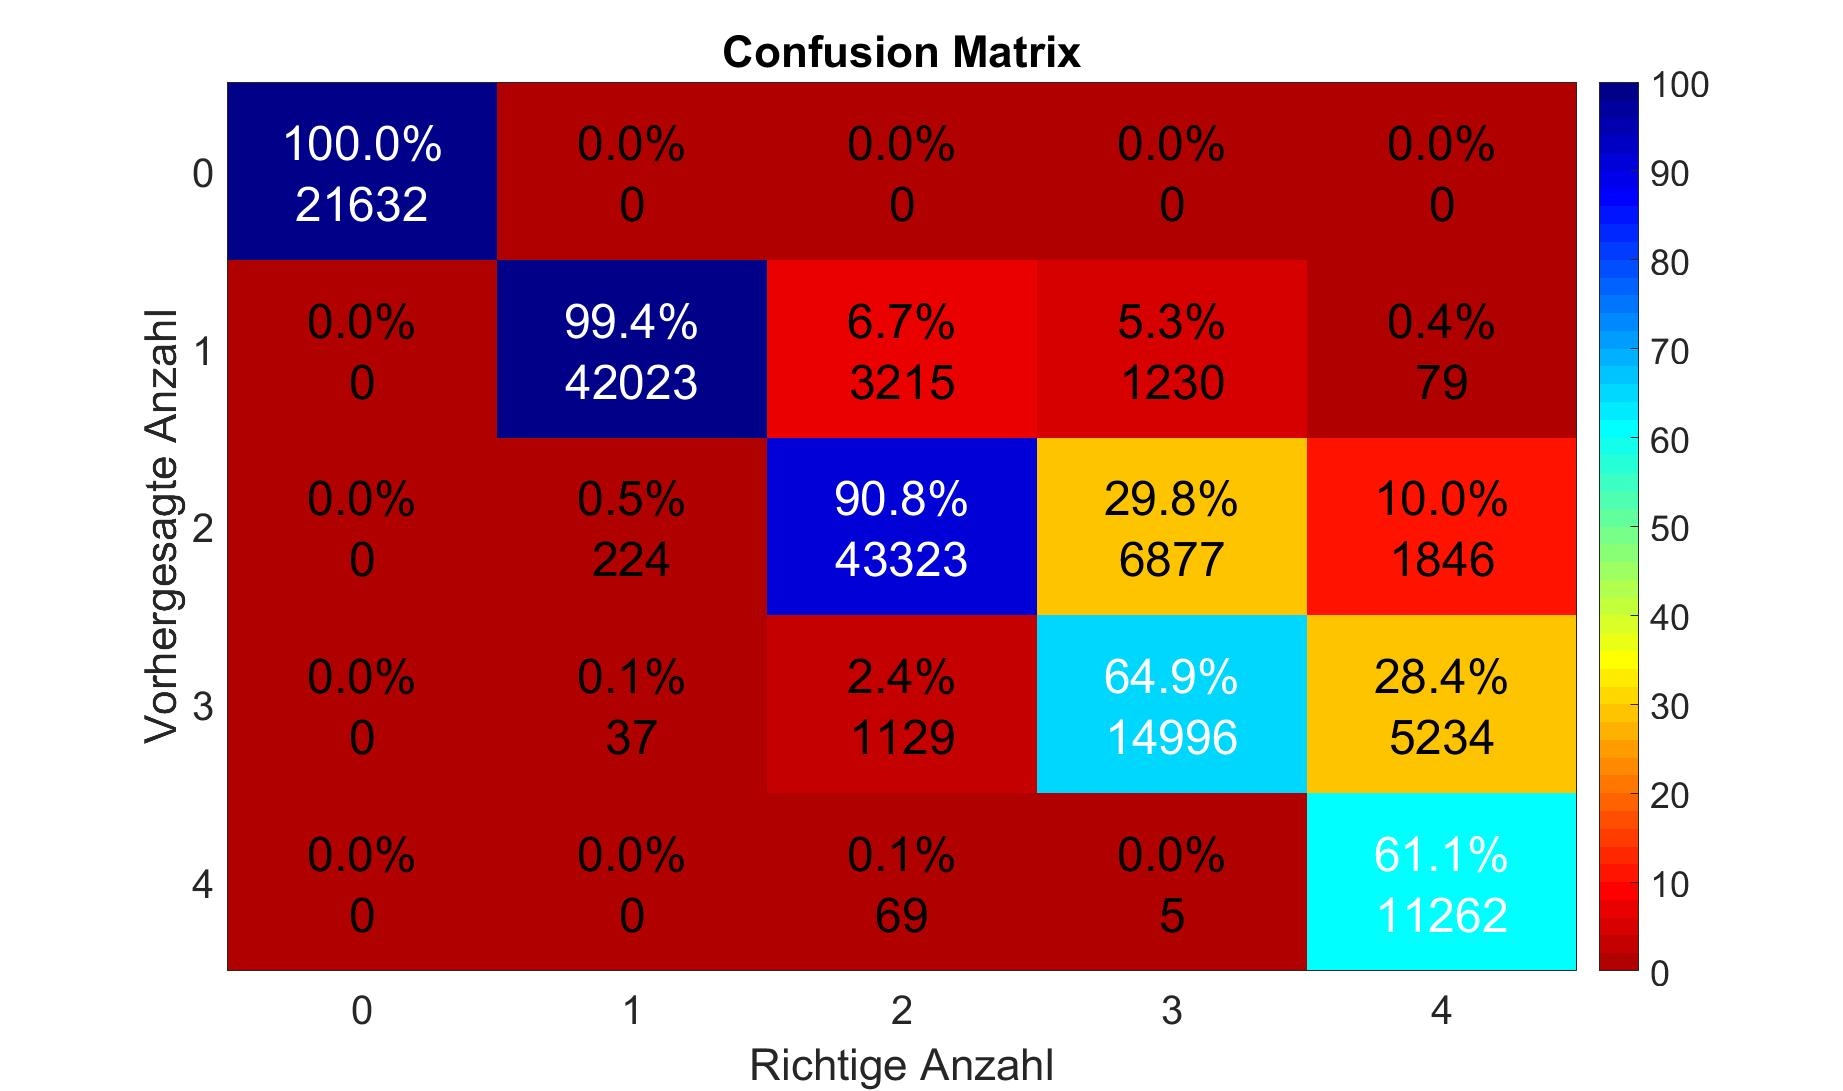
\includegraphics[width=0.55\linewidth]{fig/Profil_2m}
	\caption[Confusion Matrix Profil 2]{Confusion Matrix Profil 2}
			\label{fig:profil2}
\end{figure}
 Es wurden verhältnismäßig auch viele Frames mit vier Personen als drei Personen wahrgenommen. Das Profil 2 zeigt deutlich auf, das mit zunehmender Personenanzahl die richtige Anzahl Personen schwieriger zu detektieren ist. Die Identifikation von null bis zwei Personen gelingt in den meisten Fällen. Bei drei bis vier Personen ist die Wahrscheinlichkeit von der richtigen Personendetektion nur noch etwas über 60\%.

\subsection{Profil 3}
\label{subsec:Profil3}
Das Profil 3, dessen Confusion Matrix in Abbildung \ref{fig:profil3} dargestellt ist, besitzt eine grosse Übereinstimmung mit den trainierten Modell. In Anhang \ref{AnhangD} ist jedoch ersichtlich, dass die zwei Personenaufzüge ganz andere Eigenschaften besitzen. Es wurde jedoch keines dieser Frames für das Training verwendet.

\begin{figure}[H]
	\centering
	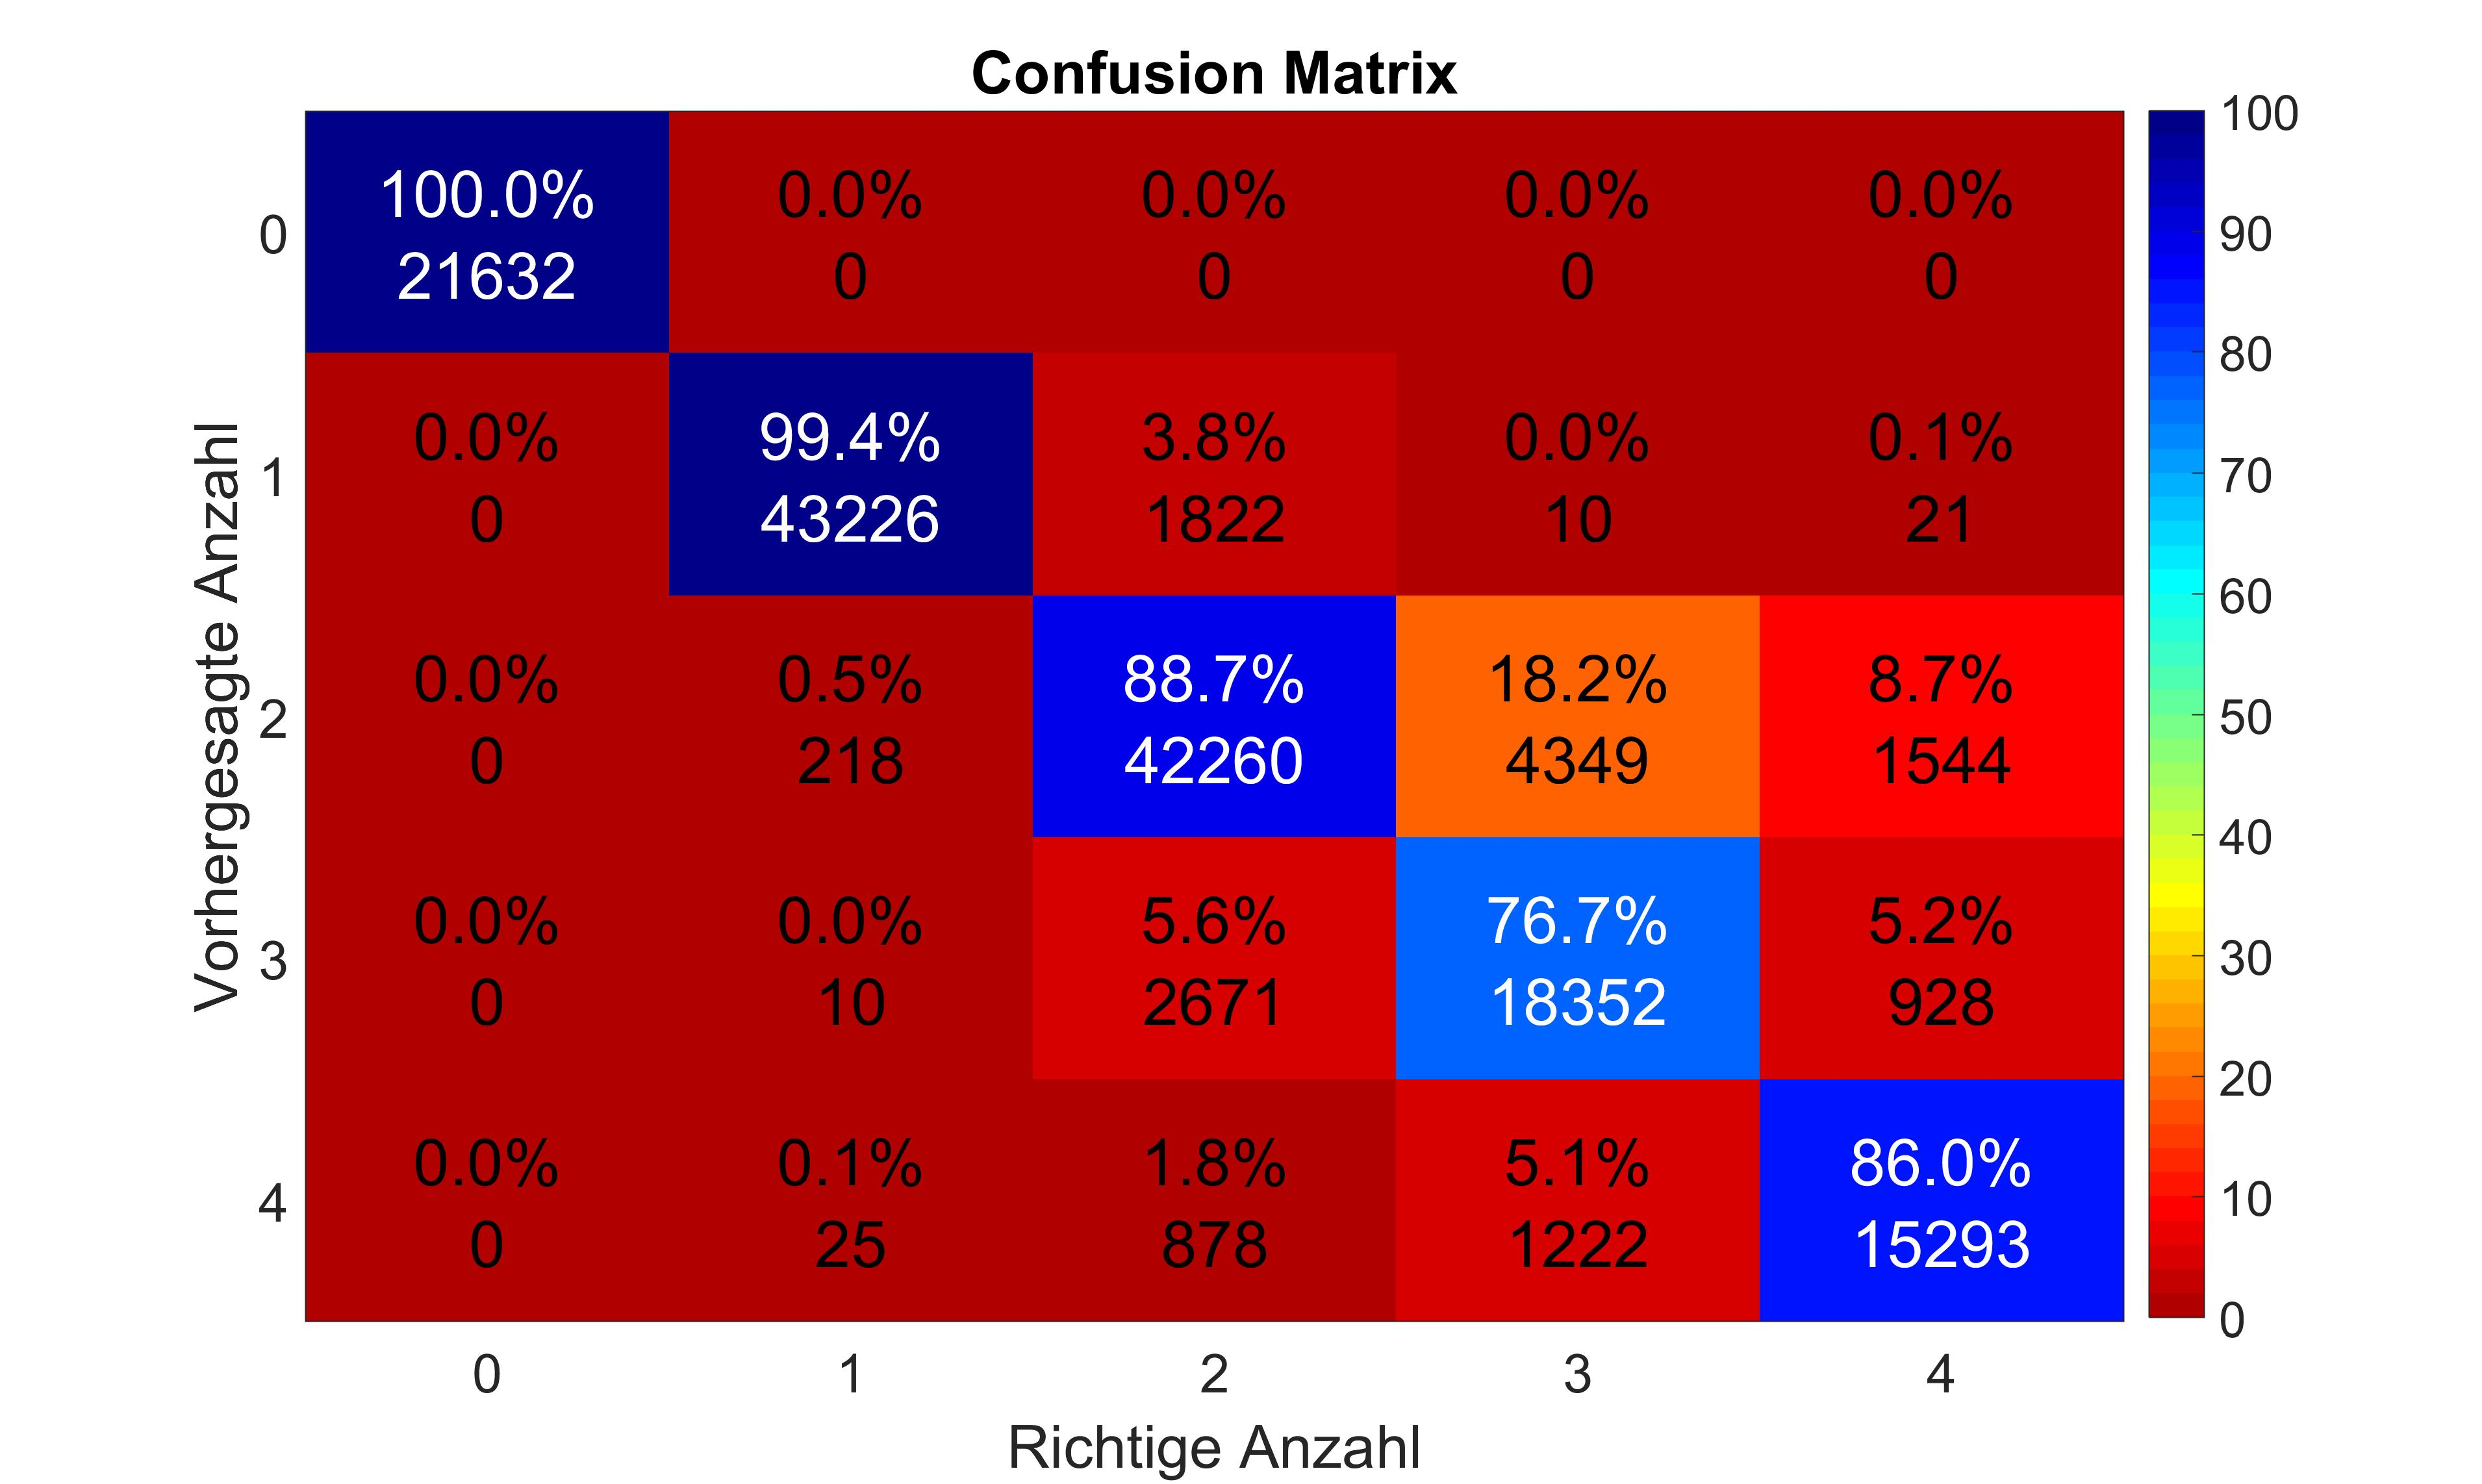
\includegraphics[width=0.55\linewidth]{fig/Profil_3m}
	\caption[Confusion Matrix Profil 3]{Confusion Matrix Profil 3}
		\label{fig:profil3}
\end{figure}

Auch hier ist die Tendenz, dass mit zunehmender Personenzahl die Übereinstimmung sinkt. Bei diesem Datensatz verursachen hauptsächlich Abschattungen durch grosse Personen und Personen am Rande des Messbereichs fehlerhafte Frames. Dennoch kann bei diesem Datensatz von einer sehr hohen Übereinstimmung  ausgegangen werden.

\subsection{Testprofil}
\label{subsec:Testprofil}
Das Testprofil in Abbildung \ref{fig:profil4} zeigt deutlich auf, welche Schwierigkeiten der Algorithmus besitzt, wenn Störquellen und Ausnahmesituationen vom \ac{CNN} verarbeitet werden. Es konnten trotz der Störeinflüsse alle 0-Personenframes richtig erkannt werden. Das Modell ist somit tolerant für Einflüsse, sofern diese nicht gravierende Änderungen zur Folge haben.
 
\begin{figure}[H]
	\centering
	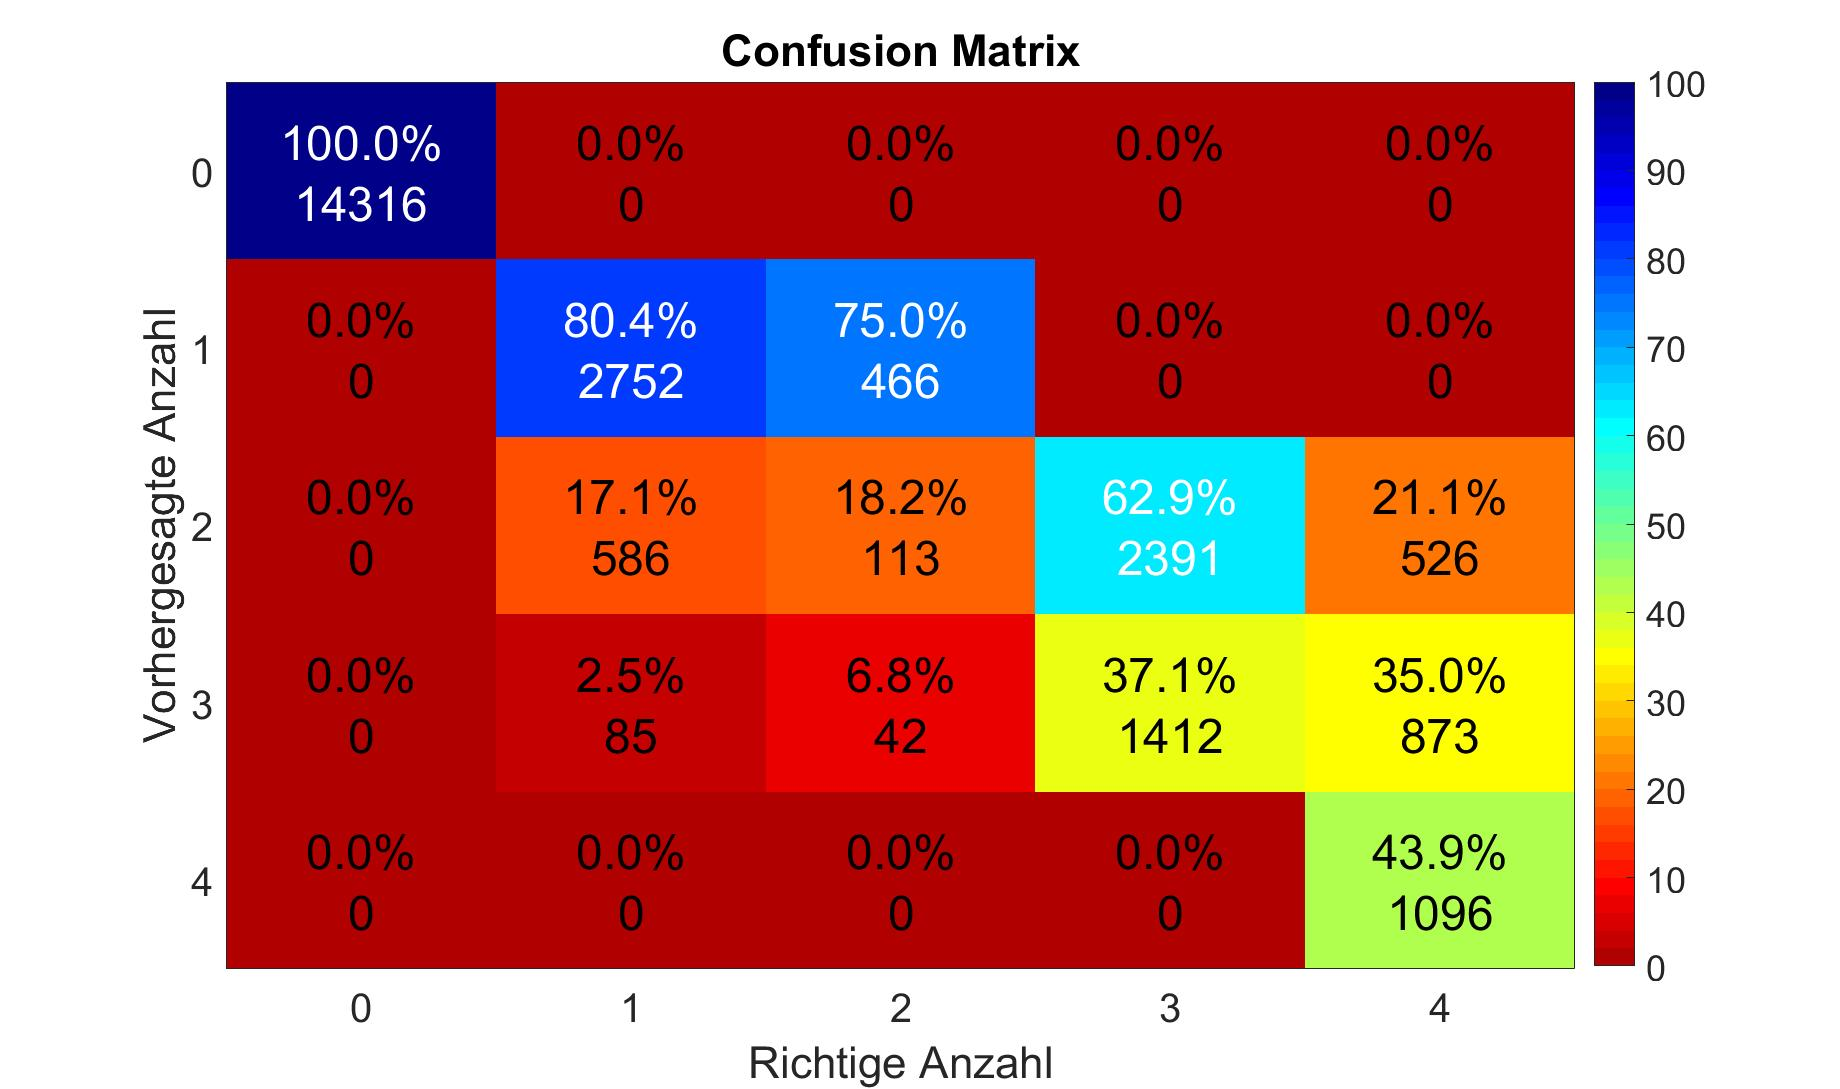
\includegraphics[width=0.55\linewidth]{fig/Testprofilm}
	\caption{Confusion Matrix Testprofil}
	\label{fig:profil4}
\end{figure}

Wenn einzelne Personen am Rand des Messbereichs stehen können diese noch identifiziert werden. Werden mehrere Personen am Rand platziert, kann das \ac{CNN} nicht mehr alle Personen richtig identifizieren. Dies erklärt die Verfehlungen oberhalb der Diagonalen.
Ein weiteres Problem ist, wenn sich neben der richtigen Anzahl Personen noch ein weitere Objekt im Messbereich befindet. Das Objekte besitzt dabei nicht Umgebungstemperatur. Dies führt dazu, dass in einigen Frames eine Person zu viel erkannt wird. Dies erklärt die Fehler unterhalb der Diagonalen. 

\newpage

\section{Echtzeitpersonenerkennung}
\label{sec:Echtzeitpersonenerkennung}
Dank der Saver-Klasse von Tensorflow lassen sich erstellte \ac{CNN}-Modelle speichern. Dabei werden alle trainierten Einstellungen in ein ckpt-File gespeichert. Diese lassen sich in ein untrainiertes \ac{CNN} laden.

Auf dieser Grundlage wurde eine Messeinheit erstellt, welche mit dem trainierten Model zur Echtzeit Personen erkennt. Die Messeinheit besteht aus einem AMG8834 Eval Kit, einem \ac{RPI3} und einer USB-Powerbank. 
In Abbildung \ref{fig:einheit1} ist die Messeinheit abgebildet. 


\begin{figure}[H]
	\centering
	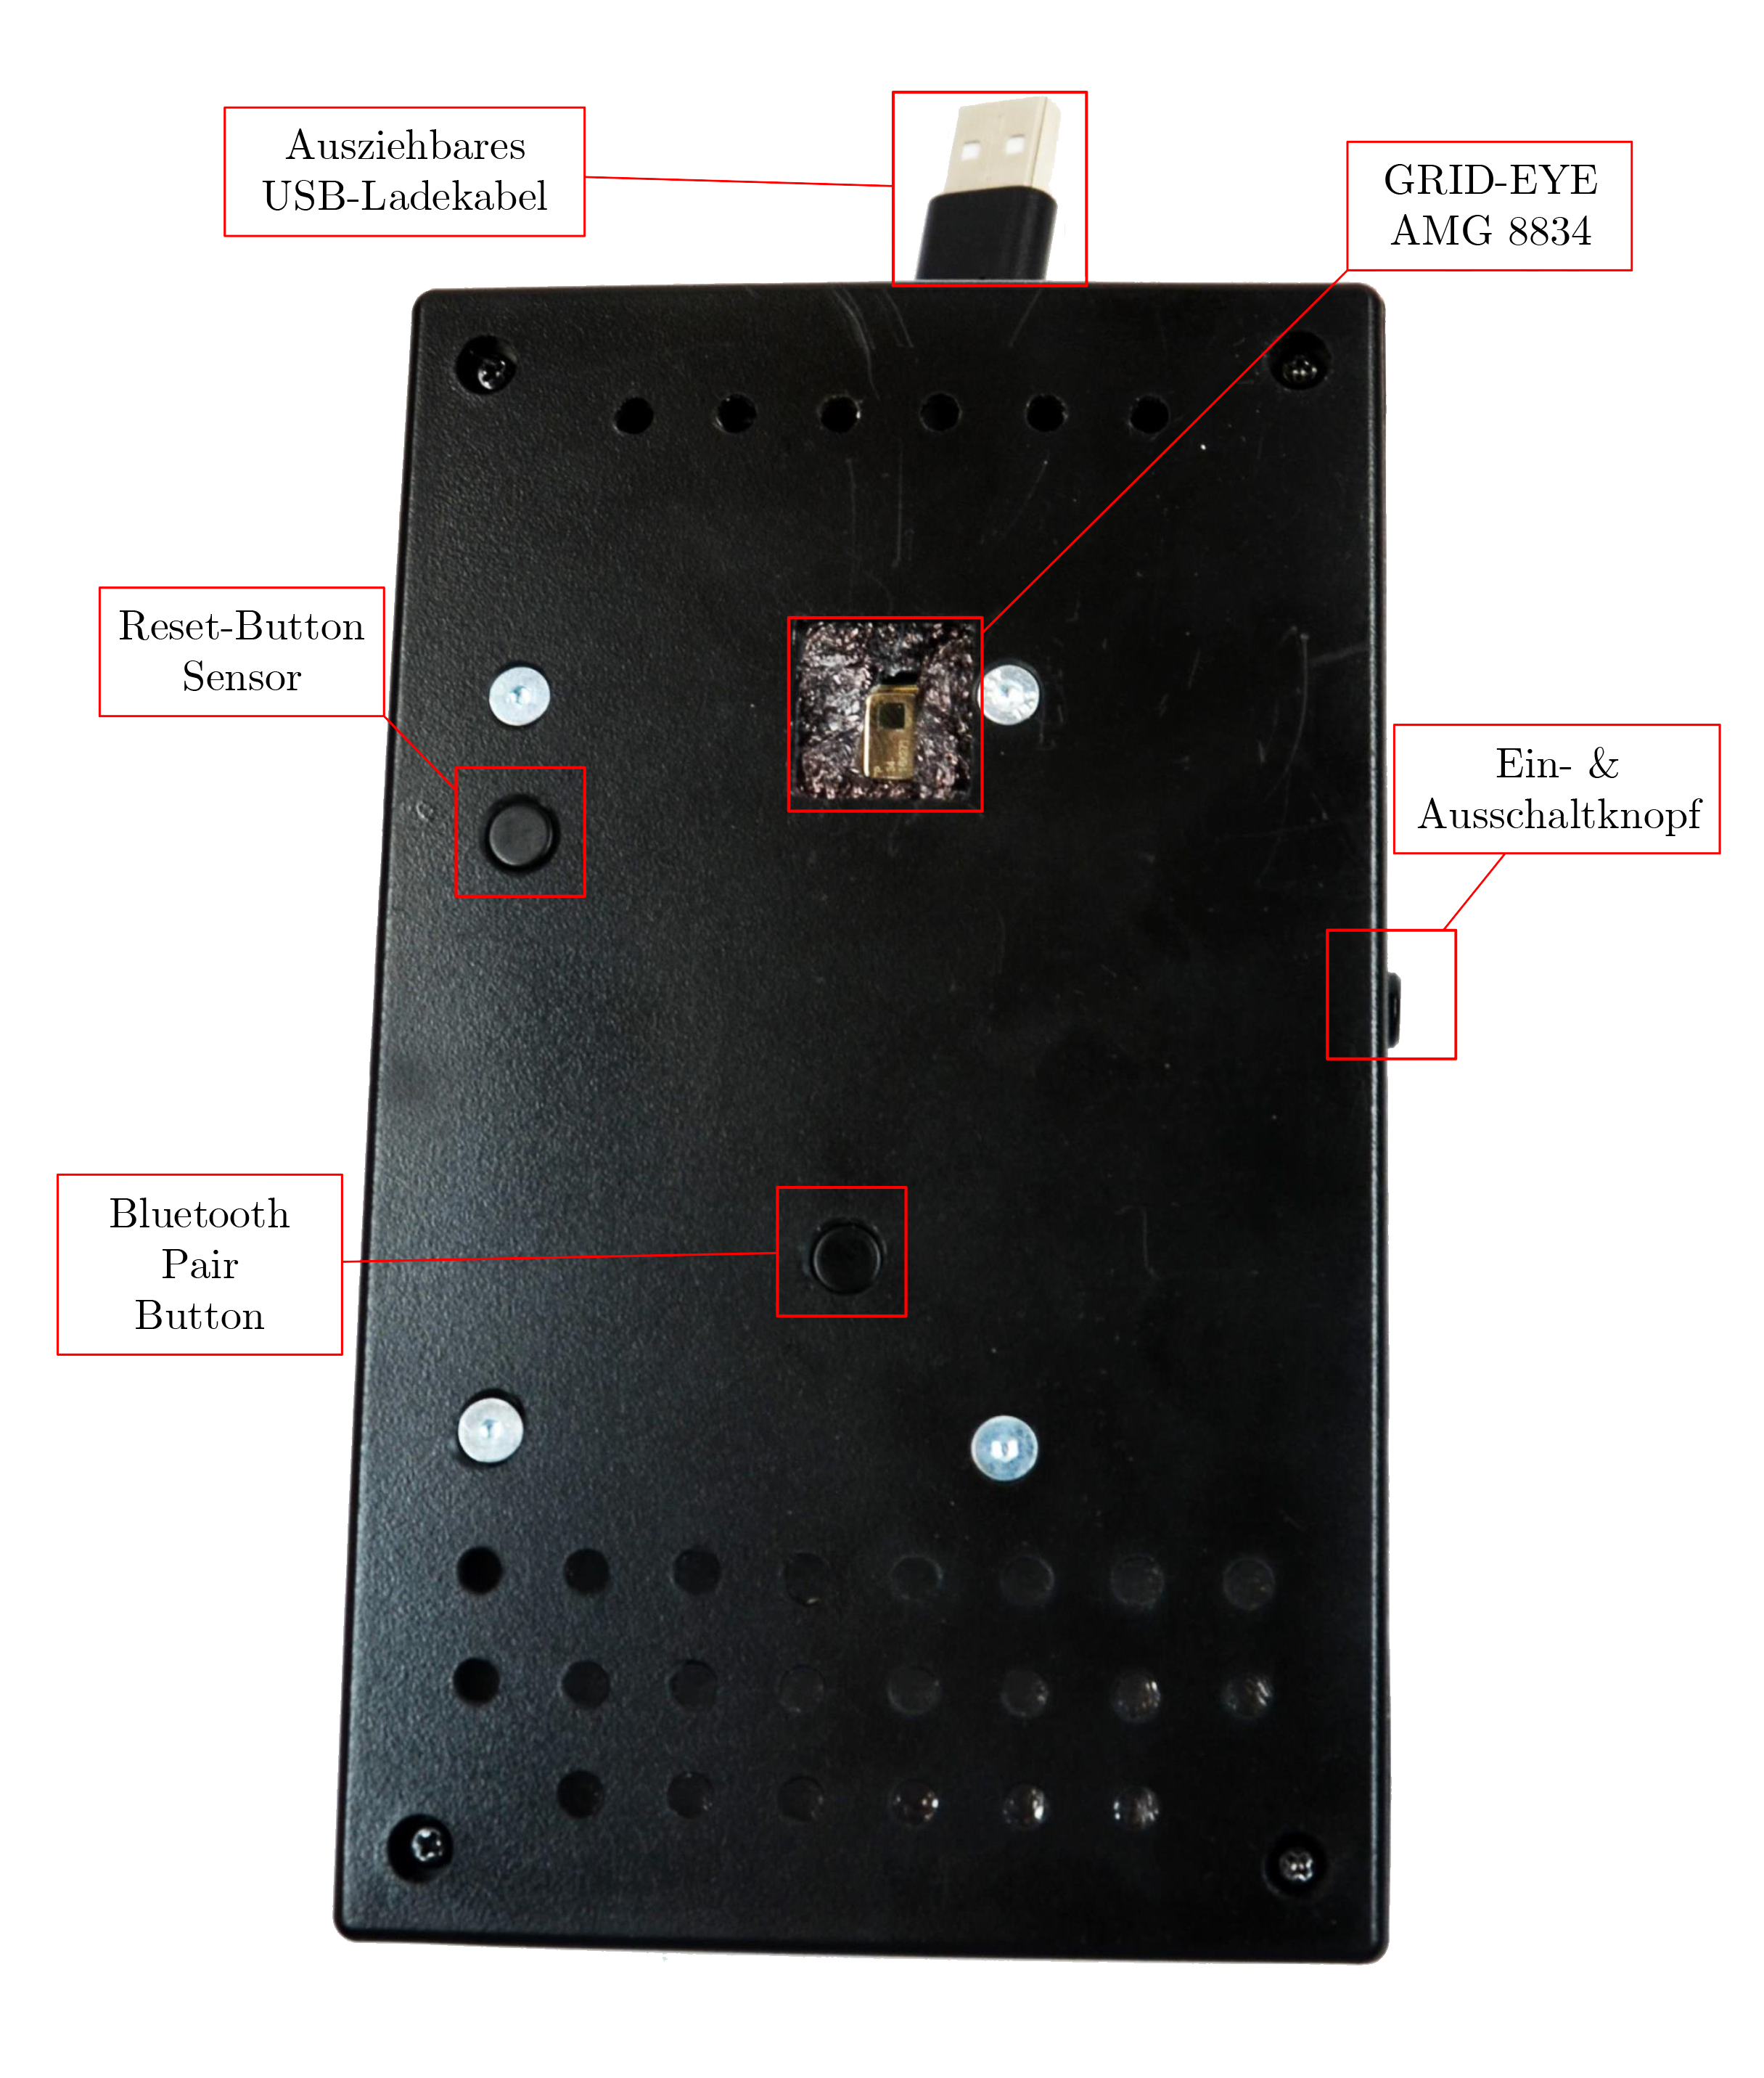
\includegraphics[width=0.85\linewidth]{fig/Echtzeitmessgeraet.jpg}
	\caption[Echtzeitmesseinheit]{Echtzeitmesseinheit}
	\label{fig:einheit1}
\end{figure}

Die Messeinheit ist für mobile Anwendungen einsetzbar. Mit der Powerbank lässt sich die Messeinheit über mehrere Stunden für Messzwecke in einem Aufzug platzieren. In Abbildung \ref{fig:einheit2}  sind die Funktionsblöcke dargestellt. Die Sensordaten werden vom AMG8834 über \ac{UART} an das \ac{RPI3} gesendet. Parallel werden diese auch über Bluetooth für die Grid-Eye App zur Verfügung gestellt, damit die Daten visualisiert werden können.

Dank einem \ac{VNC}-Server kann das \ac{RPI3} drahtlos über WLAN vom Laptop gesteuert und die Benutzeroberfläche des \ac{RPI3} auf den Laptop projiziert werden. 

\begin{figure}[H]
	\centering
	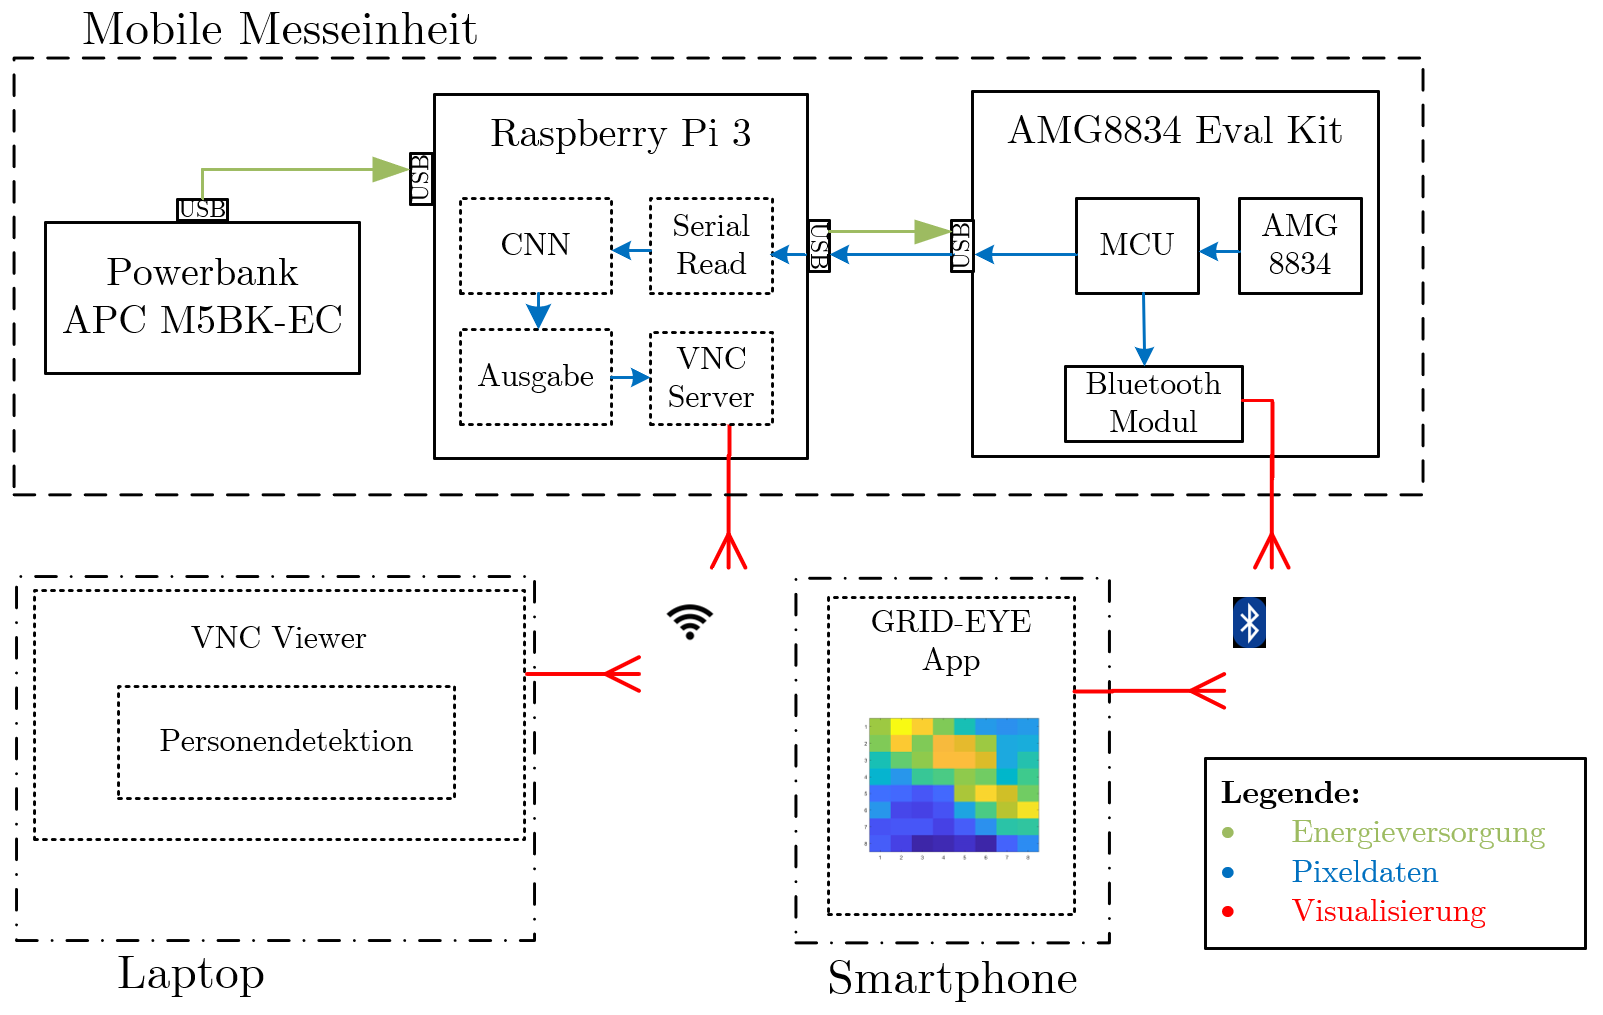
\includegraphics[width=0.9\linewidth]{fig/Messeinheit.png}
	\caption{Prinzipschema}
	\label{fig:einheit2}
\end{figure}

Die Personendetektion wird mit dem Python-Skript Persondetector\_Execution\_V1 ausgeführt. In diesem laufen parallel zwei Threads\footnote[32]{Parallel laufende Programmteile}. Der Thread Serial Read liest alle 100 ms die ankommenden Frames und bereitet diese für das \ac{CNN} vor. Im zweiten Thread wird das \ac{CNN} mit dem geladenen Modell ausgeführt. 

Die berechnete Personenanzahl wird im Zyklus von einer Sekunde ausgegeben. Dabei werden aus den zehn Frames der Median\footnote[33]{Mittelwert, unabhängig von Ausreissern} eruiert und ausgegeben. 

Auf dem \ac{RPI3} wurde das vollständige Tensorflow r1.7 installiert. Es empfiehlt sich trotzdem nicht, das Training auf dem \ac{RPI3} durchzuführen. Die Rechenzeit für ein Modell benötigt mehrere Stunden, da das \ac{RPI3} bedeutend weniger Rechenleistung bietet als übliche Computer. 

\section{Fazit}

Tensorflow bietet mit der Implementierung eines \ac{CNN} eine grosse Anzahl an Parametern und variierbaren Einstellungen, um eine Bilderkennung mittels maschinellem Lernens zu realisieren. 

Die relevantesten Punkte für die Personenerkennung sind die Frames in den Trainingssets. Es wurde mit den erstellten Datensätzen eine möglichst breite Palette an Situationen generiert, aber trotzdem lassen sich zum Teil Frames nicht differenzieren.

Die Auflösung ist in diesem Zusammenhang von grosser Bedeutung. Da nur 8x8 Pixel zur Verfügung stehen, ist die Tiefe des neuronalen Netzwerk begrenzt. Es lassen sich viele Features aus den Frames generieren, doch die Unterschiede zu anderen Objekten lassen sich nur bedingt erstellen. Vor allem an den Rändern reichen die vorhandenen Bildinformationen nicht aus um zweifelsfrei die richtige Anzahl Personen zu detektieren. 

Die Genauigkeit des Sensors streut mit 2.5 °C bedeutend. Dies ermöglicht, dass mehr unterschiedliche Frames vorhanden sind. Doch die Streuung verursacht eine grosse Messunsicherheit, welche vor allem bei Bilder zu tragen kommen, in denen mehrere Personen von unterschiedlicher Grösse nahe nebeneinander stehen. Durch die Unsicherheit lassen sich einzelne grosse Personen kaum von mehreren kleinen Personen differenzieren.






